% !TeX root = ../libro.tex
% !TeX encoding = utf8

\chapter{Introducción}\label{ch:ad-introduccion}

La detección de anomalías en series temporales consiste en el análisis de series que trata de descubrir si hay algo raro en ellas, tanto como si se señalan ciertos puntos o la serie entera. Llamamos a estos datos como \textbf{anómalos} ya que se diferencian, ya sea por forma, intensidad o cualquier otro criterio, del patrón regular esperable de las series temporales, a las que llamamos series \textbf{normales}.

En la actualidad existen varios problemas fundamentales respecto los problemas de detección de anomalías \cite{ahmed2016survey}:

\begin{enumerate}
  \item Sin modelos \textbf{universales}: los modelos realizados suelen ser muy específicos sobre el problema que resuelven, evitando una fácil traslación a un dominio de problema distinto.
  \item La falta de \textbf{datos} públicos: en la actualidad hay muy pocos \emph{datasets} etiquetados que nos permitan \textbf{validar} los modelos para poder medir su eficacia así como para poder usar técnicas de aprendizaje \textbf{supervisado}.
\end{enumerate}

Para resolver lo primero, modelamos un \textbf{sistema de detección} de series temporales anómalas muy simple basado sobre una arquitectura LSTM que puede desplegarse, a falta de que se ajuste con los parámetros ideales, en cualquier dominio donde las series normales se comportan regularmente mediante un \textbf{patrón}. Patrones como estos son esperables en series que se miden cada cierto \textbf{periodo} de tiempo como por ejemplo electrocardiogramas, sensores, servidores...

Para el segundo problema proporcionamos una serie de técnicas que nos permiten modificar series ya existentes mediante \textbf{perturbaciones}, creando así otras nuevas que pueden servir para proporcionar nuevos \emph{datasets} artificiales con ejemplos anómalos que permitan validar los modelos de detección. Aunque sean artificiales intentan suplir esta \textbf{falta de datos} para poder al menos dar una idea de cómo se comportan los modelos ante perturbaciones de las series, que están parametrizadas para ver el rendimiento a distintas escalas de valores.

Analizaremos \textbf{experimentalmente} con ejemplos como aprende y se comporta el sistema, validándolo usando los métodos comentados para alterar las series. \textbf{Analizaremos la eficacia} del sistema frente a \textbf{distintos tipos e intensidades} de alteraciones, observando la eficacia del detector y de las perturbaciones.

\chapter{Sistema LSTM para detección de series anómalas}\label{ch:ad-detector}

Supongamos que las series vienen de una distribución desconocida $\mathcal{P}$ que podemos dividir en dos tipos: las normales y las anómalas. Las normales son las señales que podemos esperar con una \textbf{probabilidad muy alta}, mientras que las anómalas son las que su \textbf{frecuencia es inusual}.

El sistema que diseñamos intenta aprender la distribución de estas señales normales, su patrón, de manera que una señal será anómala si no se parece a lo que ha aprendido el sistema. Así diferenciamos dos partes fundamentales en nuestro modelo:

\begin{enumerate}
  \item \textbf{\emph{Autoencoder LSTM}} que aprende este patrón mediante reconstrucción de la entrada.
  \item \textbf{Detector de anomalías} en base a la distribución de los errores entre las series normales y sus reconstrucciones.
\end{enumerate}

\section{Autoencoder LSTM}

El \emph{autoencoder LSTM} se encarga de aprender mediante aprendizaje \textbf{no supervisado} cómo devolver la misma señal que se proporciona como entrada, forzando al sistema a que aprenda el patrón subyacente de los datos.

Para la arquitectura de este modelo usaremos una estructura \emph{autoencoder} (\autoref{sec:autoencoder}), sin la subdimensión codificada ya que no necesitamos esta representación, que está formada por dos partes: el \textbf{codificador} (\emph{encoder}) y el \textbf{descodificador} (\emph{decoder}). El \emph{encoder} obtiene de la serie características mediante capas LSTM, cuyo tamaño va decreciendo hasta llegar al subespacio de codificación de la series, que saltaremos hasta pasar directamente al \emph{decoder} que se encarga de usar capas LSTM con tamaño creciente hasta llegar al tamaño original de las series mediante una capa completamente conectada (\emph{Dense}) que se encargará de reproducir los valores de la serie. Además todas las capas LSTM tienen como función no lineal de activación \emph{ReLU}.

Por ejemplo para un \emph{dataset} cuyas series tienen longitud 82 y solo se tiene una característica esta sería la arquitectura \autoref{fig:ad-lstm-model}. Si tuviese otra longitud o número de características lo único que cambiaría sería la dimensión de la entrada y la salida, ajustándose a la del \emph{dataset} concreto.

\begin{figure}[htpb]
  \centering
  %\hspace*{-2.5cm}
  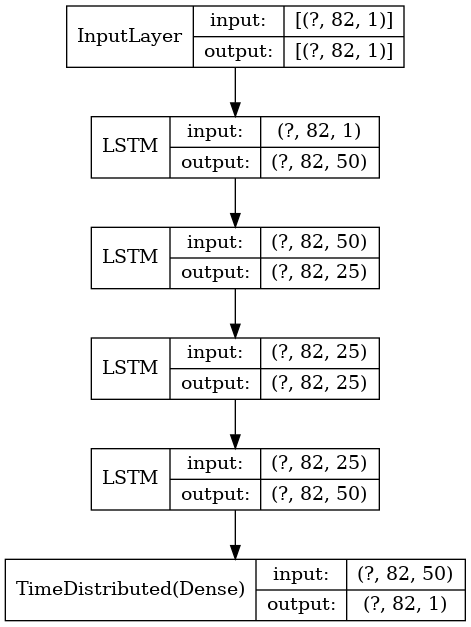
\includegraphics[width=0.35\textwidth]{model_plot}
  \caption{Arquitectura del modelo \emph{autoencoder}.}
  \label{fig:ad-lstm-model}
\end{figure}

Además se pueden modificar ciertos hiperparámetros como el número de neuronas de las capas LSTM, el parámetro de regularización de las capas, la tasa de aprendizaje, el número de épocas, el tamaño de los \emph{batches}. El método para actualizar la red es el usual de \textbf{Adam}, usando como \textbf{función de pérdida} el Error Cuadrático Medio (\emph{Mean Squared Error} \eqref{eq:mse} que es el usual para problemas de regresión y que se adecúa a nuestro problema ya que estamos prediciendo valores continuos (los de la serie) y queremos que lo minimice para que reconstruya la entrada en la salida.

\section{Detección}

La detección está basada en la \textbf{distribución de los errores} (por ejemplo, el error cuadrático medio) de distribución obtenidos en el conjunto de entrenamiento de las señales normales con las reconstrucciones del modelo LSTM. Podemos clasificar una serie \textbf{anómala} cuando el error de reconstrucción supere una cierto \textbf{umbral} fijado por nosotros. Para ser más flexibles y evitar ser tan \textbf{discriminativos}, devolveremos \textbf{probabilidades} para dar una idea más clara de cuan grave puede ser un error.

Estas probabilidades estarán basadas en la \textbf{función de probabilidad} de la distribución de los errores, de manera que para errores poco frecuentes o mucho más grandes de los vistos, tendremos una probabilidad asignada cercana a 100\% de ser anómala. Obviamente para muchas series normales se tendrán probabilidades altas, de ahí que se quiera tomar un \textbf{umbral} alto para asegurarnos que lo que se detecte sea realmente una anomalía.

La función de probabilidad como ya sabemos se puede obtener integrando la función de densidad, que \textbf{estimaremos} con una cantidad razonable de datos con cualquiera de los métodos ya existentes. Por lo que esta parte fundamentalmente se encargará de \textbf{aprender una función de densidad} basada en los errores de reconstrucción del \emph{dataset} de entrenamiento.

Cabe añadir que estamos partiendo del hecho de que solo tenemos series normales, \textbf{desconocemos} tanto la forma como la frecuencia de las anomalías que suele ser las circunstancias en muchos problemas reales, por lo que la probabilidad que devolvemos no es más que una \textbf{estimación}. Conforme se obtengan nuevas muestras se puede ir \textbf{mejorando el sistema}, incorporando la distribución de las series anómalas, ajustando así la probabilidad para que sea mucho más exacta.

Finalmente, si observamos que los errores suelen ser mucho más grandes que los de entrenamiento se podría considerar usar un umbral fijo, aunque en nuestro caso \textbf{alteraremos muy poco} las series por lo que es esperable que muchos errores puedan ser muy sutiles y verse casi como series normales, a lo que nos interesa que el intervalo de probabilidades se mueva dentro de los errores de las series normales.

\chapter{Alteraciones}\label{ch:ad-alteraciones}

Proporcionaremos cuatro tipos distintos de alteraciones para series temporales: dos basados en \textbf{ruido gaussiano} y los otros dos en la \textbf{descomposición STL}. Estas alteraciones intentan ser lo más \textbf{genéricas} posibles para poder ser aplicadas en un \textbf{alto rango} de dominios de problemas y lo más \textbf{naturales} posibles, intentando imitar las anomalías reales que se dan.

Si consideramos que a veces las anomalías como tales están consideradas así bajo un \textbf{criterio concreto} de un dominio específico del problema es muy difícil intentar tomarlas todas en cuenta; sin embargo sí hay generalmente unas pocas anomalías típicas que se suele querer detectar:

\begin{enumerate}
  \item \textbf{\emph{Pico}}: se dice que hay un \emph{pico} en la serie cuando en un periodo muy pequeño de tiempo toma un valor muy alto o muy bajo de lo usual en comparación en un entorno local.
  \item \textbf{Cambio estacional}: cuando en una serie donde se ve un patrón estacional (cada cierto periodo se repite una estructura) en uno de los periodos la intensidad de la señal cambia, aumentando o decreciendo.
  \item \textbf{Fluctuación}: cuando en la señal tiene un cambio de forma (fluctúa) en un periodo corto de tiempo, aunque no tiene por qué variar mucho en cuanto a la intensidad.
\end{enumerate}

Intentaremos reproducir estas anomalías mediante métodos que produzcan alteraciones \textbf{parecidas}, siendo además \textbf{regulables} a gusto del usuario para adaptarse a lo que se necesite.

Además, para todos las alteraciones es necesario un algoritmo que nos \textbf{seleccione un tramo de la serie} para poder aplicar la alteración. Implementamos \autoref{alg:ad-select-slice} que al pasarle una serie $X$ nos devuelve un trozo de ésta determinada por el punto donde empieza y su longitud. El algoritmo es muy flexible puesto que podemos indicar una longitud máxima y/o mínima y excluyendo los bordes hasta cierto punto. En líneas generales el algoritmo escoge el tramo aleatoriamente bajo los criterios impuestos, y siempre que sea posible según la longitud de la serie.

\begin{algorithm}[htbp]
\SetAlgoLined
  \tcp{Obtenemos la longitud máxima posible}
  $max\_length \gets \min(max\_length, X.length - 2 \cdot border)$\;
  \tcp{Escogemos un tamaño aleatorio}
  $length \gets round(distribucion\_uniforme(min\_length, max\_length))$\;
  \tcp{Ajustamos la posición máxima posible}
  $max\_pos \gets X.length - \max(border, length)$\;
  \tcp{Tomamos la posición aleatoriamente}
  $pos \gets round(distribucion\_uniforme(border, max\_pos))$\;
 \KwResult{$pos$, $length$}
 \caption{random\_slice($X$, $max\_length$, $min\_length$, $border$)}
 \label{alg:ad-select-slice}
\end{algorithm}

La posible aleatoriedad que introducimos está hecha para poder generar \textbf{muchísimas alteraciones} de golpe que sean distintas entre sí automáticamente, generando efectivamente muchas muestras anómalas para validación.

\section{Ruido gaussiano}

La distribución \textbf{normal} o \textbf{gaussiana} nos es muy útil para intentar simular un \emph{pico} ya que su forma de campana se asemeja mucho a un cambio de intensidad muy alto y es además de forma continua. Recreamos esto mediante un muestreo de la función de densidad en el intervalo $[-3 \sigma, 3 \sigma]$, obteniendo el 99.74\% de la distribución (\autoref{def:ruido-gauss}).

\begin{definicion}[Ruido gaussiano]
  Sea $\{X_t\}_{t = 1}^n$ un proceso del que se extrae una serie temporal $\{x_t\}_{t = 1}^n$, se define la perturbación de ruido gaussiano de parámetro $\sigma \in \R$, con centro $c \in N$ y longitud $\ell \in N$ tal que $c + \ell \leq n$ aplicada a la serie $\{x_t\}$ como la serie alterada $\{x_t'\}_{t = 1}^n$ dada por

  $$x_t' = \begin{cases}
    x_t + \sigma r_{t - c + 1}, & c \leq t \leq n \\
    x_t, & \text{en caso contrario.}
  \end{cases},$$

  donde $\{r_t\}_{t = 1}^\ell \subset \R$ es un muestreo de la función de densidad de la distribución gaussiana $N(0, \frac{\ell}{6})$ con $\ell$ puntos equidistantes en el intervalo $[-\frac{\ell}{2}, \frac{\ell}{2}]$.
  \label{def:ruido-gauss}
\end{definicion}

Para hacer que el muestro sea significativo, esto es, que la mayoría de puntos tomados tengan un valor no nulo, tomamos $\sigma = \ell / 6$ y se toma el in. Finalmente se multiplica todo otra vez por un parámetro $\sigma$ que se le pasa al algoritmo para controlar el grado de \textbf{intensidad} de la alteración.

Si queremos picos muy \textbf{pronunciados} solo tendremos que tomar una longitud de alteración pequeña y un $\sigma$ alto. Para otros \emph{picos} más suaves aumentamos un poco la longitud y disminuimos el $\sigma$. En cualquier caso, independientemente de la longitud total de la serie, la longitud de la perturbación no debería ser muy grande puesto que estaríamos afectando a un porcentaje mayor de la serie (ya no sería una anomalía puntual) y la perturbación se aplana ya que la desviación de la gaussiana se vuelve mayor.

Podemos ver distintos muestreos con varios tamaños y $\sigma$ en \autoref{fig:ad-ruido-gaussiano}, observándose que efectivamente se tiene un muestreo correcto, con intensidad moldeable por $\sigma$ y que según la longitud deseada se puede hacer un cambio más brusco o suave.

\begin{figure}[htpb]
  \centering
  %\hspace*{-2.5cm}
  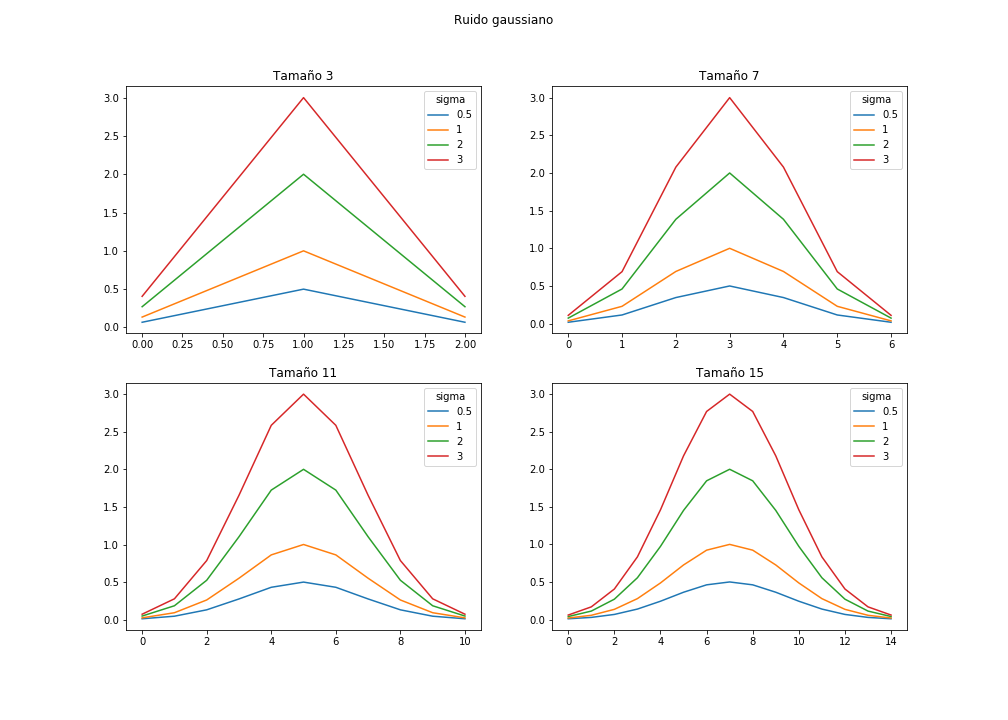
\includegraphics[width=.9\textwidth]{ej_gaussian_noise}
  \caption{Muestreos de la distribución gaussiana con distintos tamaños y $\sigma$.}
  \label{fig:ad-ruido-gaussiano}
\end{figure}

Finalmente, la serie alterada que se devuelve es la original $x$ sumando al tramo seleccionado anteriormente el muestreo que hemos obtenido. Se ha incluido también una opción para que aleatoriamente se reste en vez de sumar, para crear un pico invertido.

Tomando el \emph{dataset} \emph{Beef} de \cite{bagnall2020ts}, representamos varios ejemplos de las series con las perturbaciones aplicadas, escogiendo longitudes aleatorias en $[3, 40]$ y $\sigma$ en $[0.7, 3]$ en \autoref{fig:ad-ej-ruido}. Vemos como tenemos un amplio rango de distintas perturbaciones, con picos muy empinados o más pequeños y otras más suaves.

\begin{figure}[htpb]
  \centering
  %\hspace*{-2.5cm}
  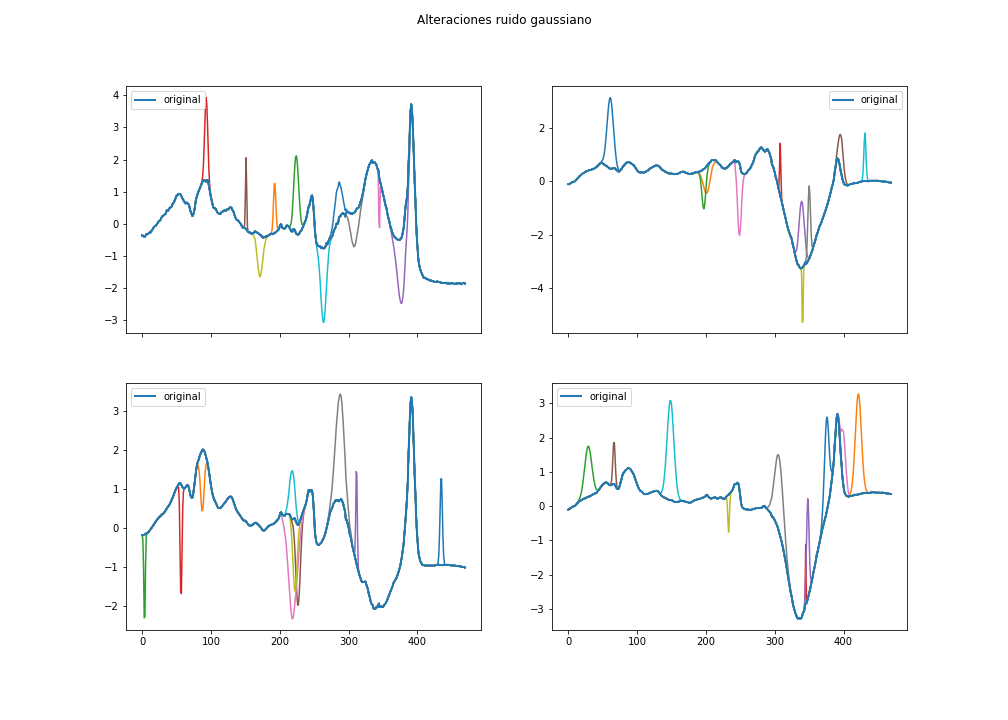
\includegraphics[width=.9\textwidth]{ej_gaussian_noise2}
  \caption{Perturbaciones con ruido gaussiano con distintas longitudes y $\sigma$ en el dataset \emph{Beef}.}
  \label{fig:ad-ej-ruido}
\end{figure}

\section{Pulso gaussiano-sinusoidal}

Introducimos la alteración de \textbf{pulso gaussiano-sinusoidal} como alteración de la forma de la señal, imitando una \textbf{fluctuación} en el tramo de la señal. Este pulso no es nada más que un pulso electromagnético con forma sinusoidal que es amortiguado con una gaussiana, es decir, una señal sinusoidal que se multiplica por la función de densidad de una gaussiana (\autoref{def:pulso-gaussiano-sinusoidal}).

\begin{definicion}[Pulso gaussiano-sinusoidal]
  Sea $\{X_t\}_{t = 1}^n$ un proceso del que se extrae una serie temporal $\{x_t\}_{t = 1}^n$, se define la perturbación de pulso gaussiano-sinusoidal de parámetro $\sigma \in \R$, con frecuencia $f \in \R^{+}$, centro $c \in N$ y longitud $\ell \in N$ tal que $c + \ell \leq n$ aplicada a la serie $\{x_t\}$ como la serie alterada $\{x_t'\}_{t = 1}^n$ dada por

  $$x_t' = \begin{cases}
    x_t + \sigma p_{t - c + 1} r_{t - c + 1}, & c \leq t \leq n \\
    x_t, & \text{en caso contrario.}
  \end{cases},$$

  donde $\{r_t\}_{t = 1}^\ell \subset \R$ es un muestreo de la función de densidad de la distribución gaussiana $N(0, \frac{\ell}{6})$ con $\ell$ puntos equidistantes en el intervalo $[-\frac{\ell}{2}, \frac{\ell}{2}]$ y $\{p_t\}_{t = 1}^\ell \subset \R$ es un muestreo de la función $\cos$ con $\ell$ puntos equidistantes en el intervalo $[-2\pi f, 2\pi f]$.
  \label{def:pulso-gaussiano-sinusoidal}
\end{definicion}

Igual que hacíamos antes, se toma el muestreo y se multiplica por el $\sigma$ aplicado, sumando esta alteración al tramo elegido aleatoriamente. La frecuencia $f$ debe ser tomada respecto a la longitud de la perturbación $\ell$ para que el muestreo sea correcto.

Unos cuantos ejemplos de pulsos gaussianos-sinusoidal los tenemos en \autoref{fig:ad-pulso-gaussiano}, que indican que por lo menos necesitamos un tamaño considerable para que el muestreo sea significativo (que se muestre el carácter sinusoidal) y en cualquier caso podemos modificar la intensidad con $\sigma$.

\begin{figure}[htpb]
  \centering
  %\hspace*{-2.5cm}
  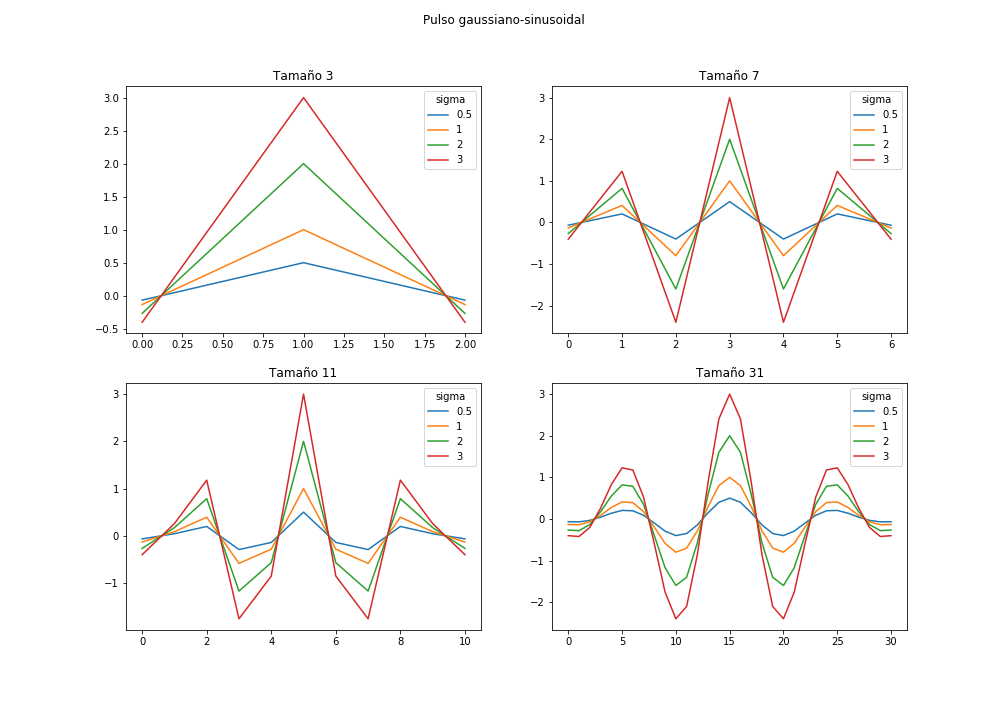
\includegraphics[width=.9\textwidth]{ej_gaussian_pulse}
  \caption{Ejemplos de pulsos gaussianos-sinusoidales con distintos tamaños y $\sigma$.}
  \label{fig:ad-pulso-gaussiano}
\end{figure}

Finalmente en el \emph{dataset} \emph{ECG5000} de \cite{bagnall2020ts}, repetimos ejemplificando las perturbaciones tomando longitudes en el intervalo $[7, 11]$ y con $\sigma$ en $[0.5, 1.5]$ en \autoref{fig:ad-ej-pulso}. Cambiamos efectivamente la forma de la señal introduciendo pequeñas oscilaciones de los valores, que pueden ser más o menos bruscas según se necesite.

\begin{figure}[htpb]
  \centering
  %\hspace*{-2.5cm}
  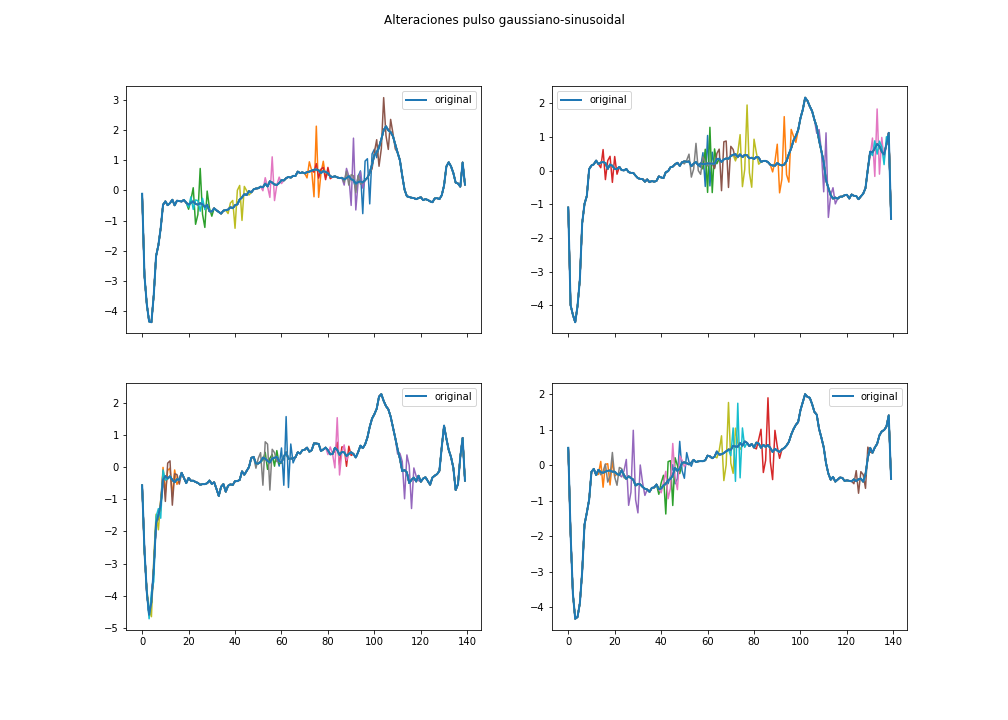
\includegraphics[width=.9\textwidth]{ej_gaussian_pulse2}
  \caption{Perturbaciones con pulso gaussiano-sinusoidal con distintas longitudes y $\sigma$ en el dataset \emph{ECG5000}.}
  \label{fig:ad-ej-pulso}
\end{figure}

\section{Modificación STL}

Para intentar emular el \textbf{cambio estacional} utilizaremos la técnica de descomposición STL y modificaremos las series de \textbf{tendencia} y \textbf{estacionalidad}.

Estas técnicas están dirigidas especialmente cuando el \emph{dataset} muestra cierta tendencia estacional para poder \textbf{descomponerla} correctamente, considerando que los métodos necesitan el \textbf{periodo} de esta estacionalidad que tendremos que estimar más o menos para poder realizar las modificaciones bien.

Para poder hacer perturbaciones de este estilo que se apliquen correctamente hemos creado un \emph{dataset} artificial formado por muestreos de 100 valores de la función \textbf{coseno}, que aporta la componente \textbf{estacional}. Después se ha hecho un muestreo del intervalo $[0, 1]$ con 100 puntos equidistantes, sumándolo a la serie para darle la \textbf{tendencia}. A continuación se ha añadido ruido gaussiano aleatorio para darle ruido y que las muestras sean diferentes; y finalmente se han estandarizado.

Visualizamos unas 50 muestras \autoref{fig:ad-cosenos} y comprobamos que efectivamente que tenemos la función coseno con una tendencia al alza y con cierto ruido para cada serie.

\begin{figure}[htpb]
  \centering
  %\hspace*{-2.5cm}
  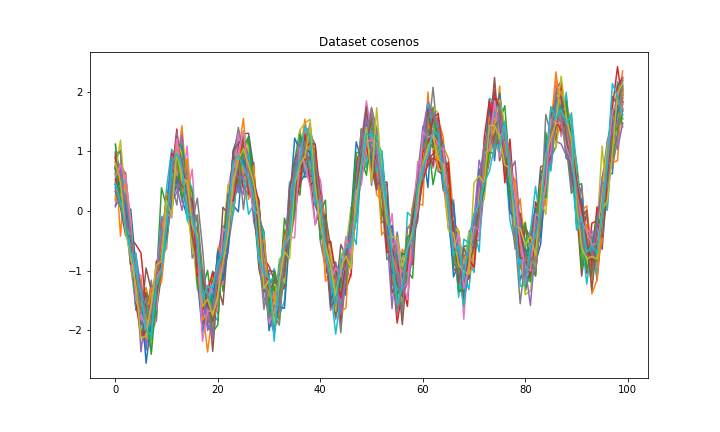
\includegraphics[width=.7\textwidth]{cosenos}
  \caption{\emph{Dataset} de cosenos.}
  \label{fig:ad-cosenos}
\end{figure}

\subsection{Estacionalidad}

Esta modificación consiste simplemente en obtener la parte de estacionalidad de la descomposición STL de la serie y en amplificarla o disminuirla multiplicando por el parámetro $\sigma$, haciendo un cambio en la serie pero \textbf{sin cambiar su forma} (\autoref{def:stl-estacionalidad})

\begin{definicion}[Pulso gaussiano-sinusoidal]
  Sea $\{X_t\}_{t = 1}^n$ un proceso del que se extrae una serie temporal $\{x_t\}_{t = 1}^n$, consideramos la descomposición STL con periodo $S$ de la serie como

  $$x_t = m_t + s_t + Y_t, \; \forall t = 0, \ldots, n,$$

  Se define la perturbación de estacionalidad de parámetro $\sigma \in \R$, con centro $c \in N$ y longitud $\ell \in N$ tal que $c + \ell \leq n$ aplicada a la serie $\{x_t\}$ como la serie alterada $\{x_t'\}_{t = 1}^n$ dada por

  $$x_t' = \begin{cases}
    m_t + \sigma s_{t} + Y_t, & c \leq t \leq n \\
    m_t + s_t + Y_t, & \text{en caso contrario.}
  \end{cases}.$$
  \label{def:stl-estacionalidad}
\end{definicion}

Ejemplificamos lo que estamos haciendo en \autoref{fig:ad-seasonal2}, probando con distintos periodos y $\sigma$. Notamos como si se toma un valor de periodo incorrecto se pueden obtener resultados no deseados, en este caso el periodo que parece que mejor encuentra la descomposición es 13. Por otro lado vemos como conseguimos lo que queremos, teniendo en cuenta que la serie original está con $\sigma = 1$ amplificamos cuando $\sigma > 1$ y amortiguamos con $\sigma < 1$.

\begin{figure}[htpb]
  \centering
  %\hspace*{-2.5cm}
  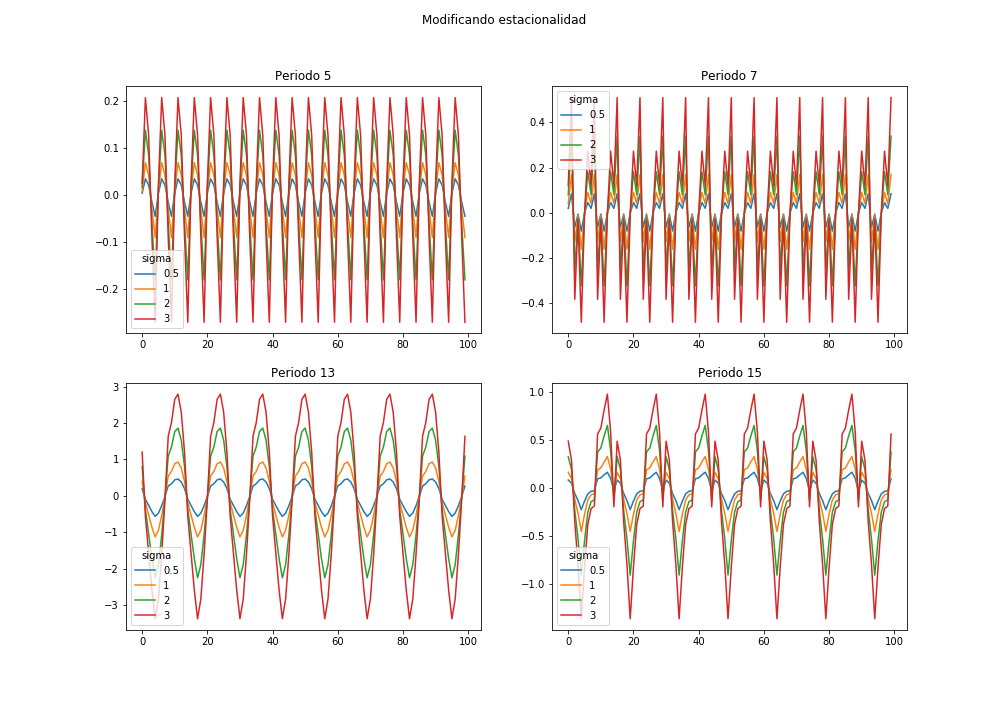
\includegraphics[width=.95\textwidth]{ej_season2}
  \caption{Modificación de la estacionalidad de cosenos.}
  \label{fig:ad-seasonal2}
\end{figure}

Para ver el efecto en las series completas, cogemos el periodo de 13 que hemos visto que recoge bien la descomposición y variamos la longitud de las perturbaciones entre $[3, 13]$ y $\sigma$ entre $[0, 2.5]$ para que pueda amplificar o disminuir la señal, cuyos resultados están en \autoref{fig:ad-seasonal}

\begin{figure}[htpb]
  \centering
  %\hspace*{-2.5cm}
  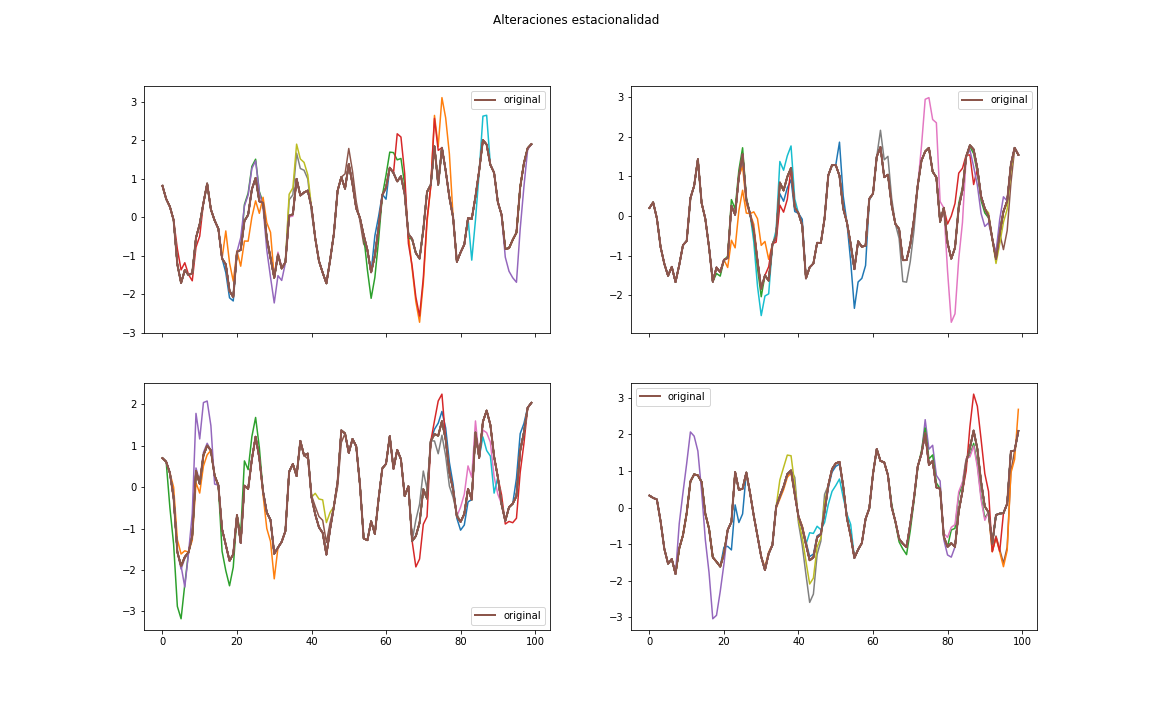
\includegraphics[width=.95\textwidth]{ej_season}
  \caption{Modificación de estacionalidad con distintas longitudes y $\sigma$.}
  \label{fig:ad-seasonal}
\end{figure}

En este caso vemos que son muy variadas las perturbaciones pero que generalmente cumplen su propósito al aumentar o decrementar la serie en ciertos momentos sin alterar la forma de las señales.

\subsection{Tendencia}

Procedemos igual que la estacionalidad, pero en este caso cambiamos la tendencia. Hacemos la descomposición STL de la serie y aumentamos o amortiguamos multiplicando por un parámetro $\sigma$ que cambia la serie sin modificar su forma (\autoref{def:stl-tendencia}).

\begin{definicion}[Pulso gaussiano-sinusoidal]
  Sea $\{X_t\}_{t = 1}^n$ un proceso del que se extrae una serie temporal $\{x_t\}_{t = 1}^n$, consideramos la descomposición STL con periodo $S$ de la serie como

  $$x_t = m_t + s_t + Y_t, \; \forall t = 0, \ldots, n,$$

  Se define la perturbación de tendencia de parámetro $\sigma \in \R$, con centro $c \in N$ y longitud $\ell \in N$ tal que $c + \ell \leq n$ aplicada a la serie $\{x_t\}$ como la serie alterada $\{x_t'\}_{t = 1}^n$ dada por

  $$x_t' = \begin{cases}
    \sigma m_t + s_{t} + Y_t, & c \leq t \leq n \\
    m_t + s_t + Y_t, & \text{en caso contrario.}
  \end{cases}.$$
  \label{def:stl-tendencia}
\end{definicion}

Algunos ejemplos los tenemos en \autoref{fig:ad-trend} que volvemos a probar con varios periodos y $\sigma$. Se confirma que el periodo 13 es el que mejor se ajusta a la descomposición, y que la tendencia aumenta o disminuye según $\sigma$ considerando que el caso original es $\sigma = 1$.

\begin{figure}[htpb]
  \centering
  %\hspace*{-2.5cm}
  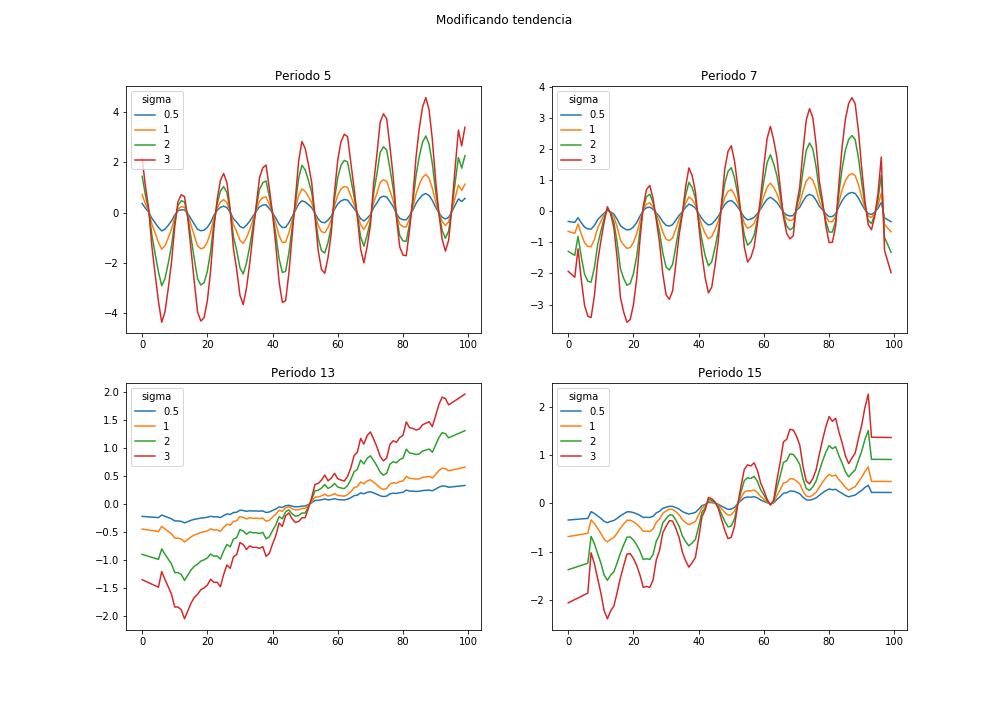
\includegraphics[width=.95\textwidth]{ej_trend}
  \caption{Modificación de la tendencia de cosenos.}
  \label{fig:ad-trend}
\end{figure}

Finalmente vemos los efectos al alterar la tendencia en \autoref{fig:ad-ej-trend2} cambiando la longitud en $[3, 13]$ y $\sigma$ en $[0, 5]$ (hemos aumentado el sigma para que se notasen mejor los efectos). Notamos que la tendencia se suaviza o potencia conforme $\sigma$, por lo que hemos conseguido los efectos deseados.

\begin{figure}[htpb]
  \centering
  %\hspace*{-2.5cm}
  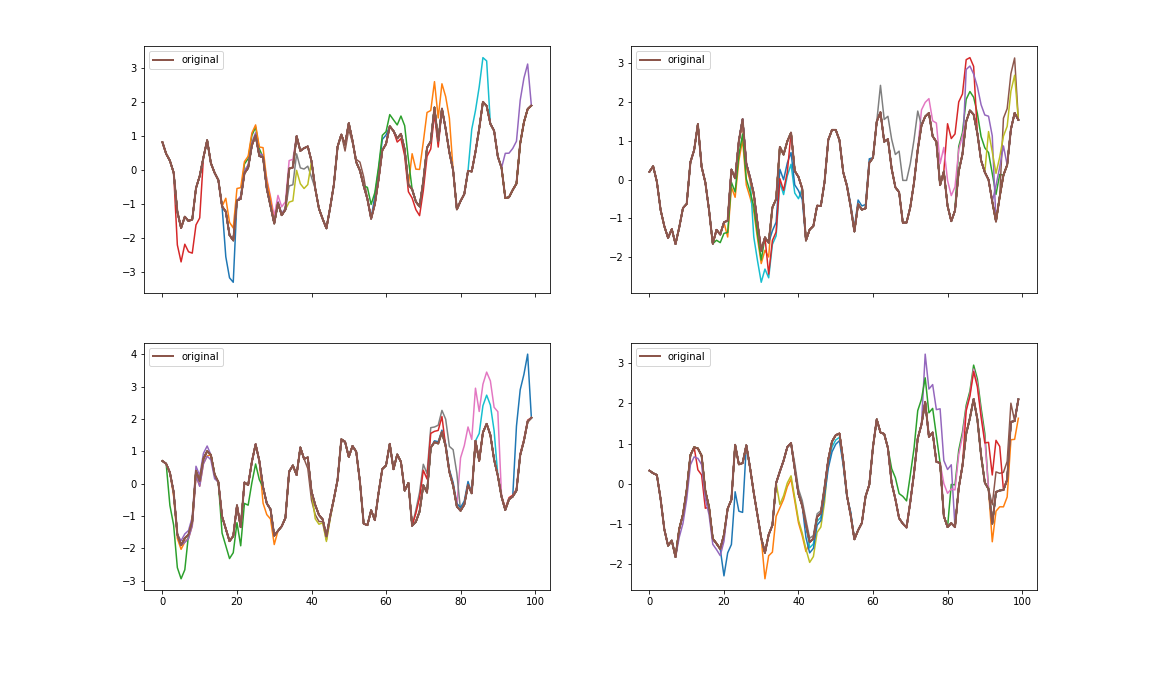
\includegraphics[width=.95\textwidth]{ej_trend2}
  \caption{Modificación de tendencia con distintas longitudes y $\sigma$.}
  \label{fig:ad-ej-trend2}
\end{figure}

Cabe añadir que se consigue un efecto parecido tanto en \textbf{tendencia} como en \textbf{estacionalidad} al estar cambiando la intensidad de una parte de la serie sin cambiar su forma, pero los cambios son un poco distintos: con la estacionalidad se puede cambiar las partes más grandes a más, y las más pequeñas a menos; con la tendencia cambia todo a más o a menos independientemente, solo importa la parte de la tendencia.

\chapter{Experimentación}\label{ch:ad-experimentacion}

Comprobaremos \textbf{empíricamente} el sistema de detección y los métodos de perturbación introducidos mediante la experimentación en un \emph{dataset} real para probar los ruidos gaussianos, y un \emph{dataset} sintético con tendencia y estacionalidad clara para probar los basados en la descomposición STL.

\section{Dataset real}

\subsection{Descripción}

Escogemos el \emph{dataset} \emph{TwoLeadECG} de \cite{bagnall2020ts} que originalmente viene de un problema de clasificación de varias señales de electrocardiogramas. Mezclamos la partición existente, hacemos nosotros una división 80/20\% y nos quedamos solo con la clase 0 que consideramos nuestra clase normal; el resto se consideran series anómalas que también podremos usar para validar el modelo.

Inspeccionamos 10 series del \emph{dataset} para ver si ciertamente hay algún patrón normal que muestren las series en \autoref{fig:ad-dataset-two}. Efectivamente hay una forma clara que nos muestra que es posible que nuestro modelo pueda aprenderla.

\begin{figure}[htpb]
  \centering
  %\hspace*{-2.5cm}
  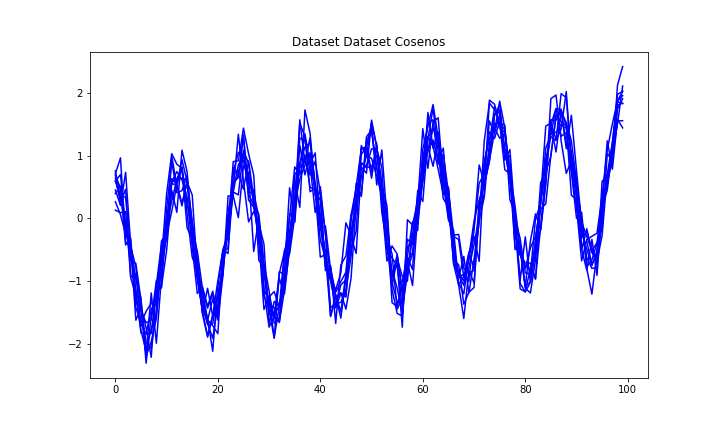
\includegraphics[width=.8\textwidth]{dataset-two}
  \caption{Algunas series de \emph{TwoLeadECG}.}
  \label{fig:ad-dataset-two}
\end{figure}

\subsection{Entrenamiento}

Usando la arquitectura comentada previamente entrenamos el modelo durante 300 épocas que después de varias pruebas comprobamos que una buena configuración nos resulta con un número de neuronas a $[50, 25, 25, 50]$ (una cantidad bastante baja y razonable en cuestión de tiempo de entrenamiento), sin regularización (provoca que aumente mucho la función de pérdida hasta desbordarse), con una tasa de aprendizaje de $0.001$ (para evitar ciertos problemas de convergencia encontrados), tamaño de \emph{batch} de 128 y con un conjunto de validación usando el 10\%.

Mostramos el resultado del entrenamiento de la función de pérdida MSE en \autoref{fig:ad-entrenamiento}. Realiza un buen entrenamiento sin sobreajuste (Val y Train están juntas), donde converge rápidamente y hemos ido siguiendo entrenando para que se ajustase lo mejor posible al patrón de las series.

\begin{figure}[htpb]
  \centering
  %\hspace*{-2.5cm}
  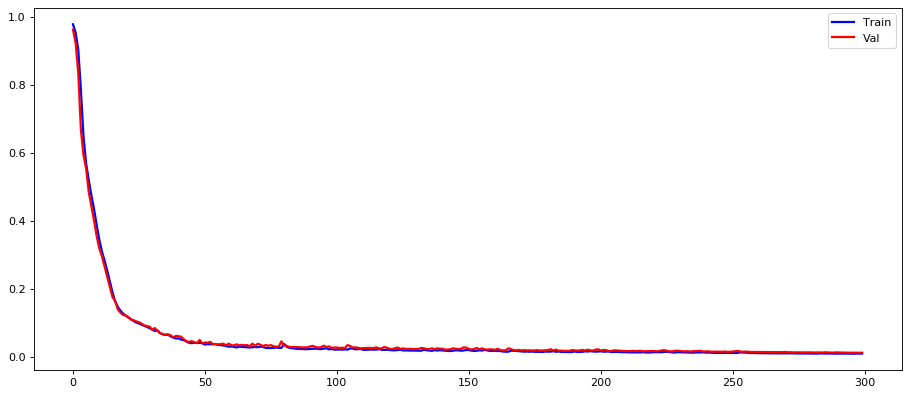
\includegraphics[width=.8\textwidth]{training_model}
  \caption{Entrenamiento del modelo LSTM.}
  \label{fig:ad-entrenamiento}
\end{figure}

Para validar los resultados veamos algunas series tanto en \emph{train} como en \emph{test} junto con sus reconstrucciones para ver que tal se comporta el modelo.
Mostramos cuatro reconstrucciones de \emph{train} en \autoref{fig:ad-reconstruccion-two-train} y cuatro de \emph{test} en \autoref{fig:ad-reconstruccion-two-test}.

En general vemos que las reconstrucciones son casi idénticas, habiendo un poco de diferencia en el primer tramo de las series, que si bien no se ajusta exactamente está bastante cerca. Después de varias configuraciones no se ha conseguido perfilar totalmente, por lo que el resultado obtenido nos parece correcto.

\begin{figure}[htpb]
  \centering
  %\hspace*{-2.5cm}
  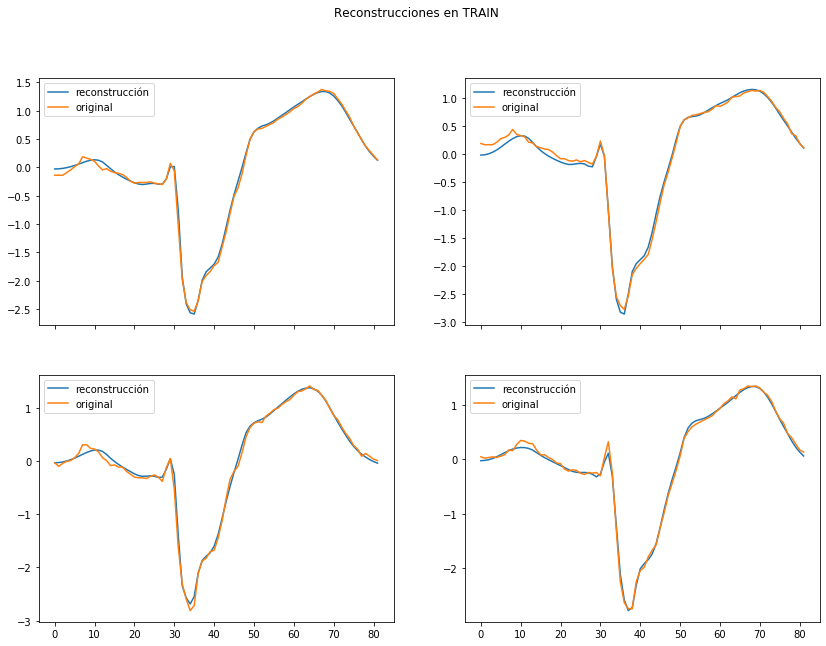
\includegraphics[width=.8\textwidth]{two_reconstruccion}
  \caption{Reconstrucciones en \emph{train}.}
  \label{fig:ad-reconstruccion-two-train}
\end{figure}

\begin{figure}[htpb]
  \centering
  %\hspace*{-2.5cm}
  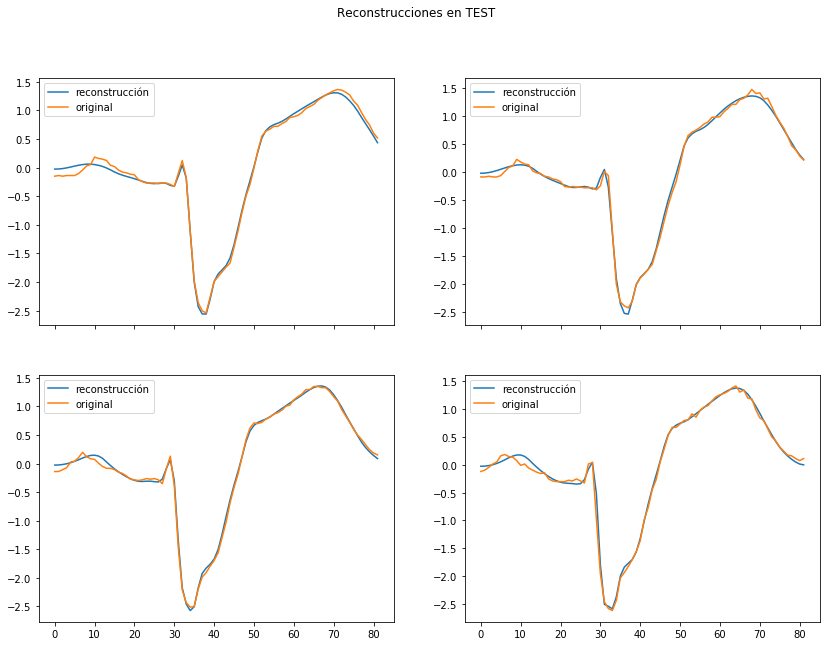
\includegraphics[width=.8\textwidth]{two_reconstruccion_test}
  \caption{Reconstrucciones en \emph{test}.}
  \label{fig:ad-reconstruccion-two-test}
\end{figure}

Ahora pasamos a estudiar la distribución de errores MSE entre las series y sus reconstrucciones con el modelo, tanto en \emph{train} como en \emph{test} (\autoref{fig:ad-hist-two}). A partir de estos datos usamos una estimación de la función de densidad que representamos también.

\begin{figure}[htpb]
  \centering
  %\hspace*{-2.5cm}
  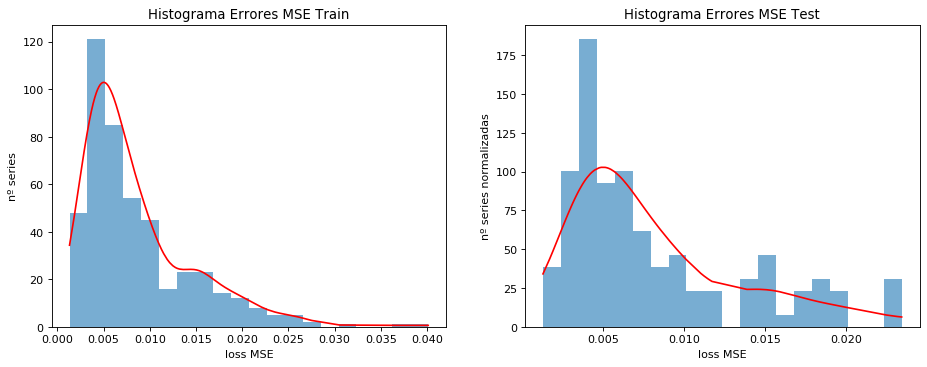
\includegraphics[width=1.\textwidth]{two-hists}
  \caption{Histogramas de error en \emph{train} y \emph{test}.}
  \label{fig:ad-hist-two}
\end{figure}

Observamos que los errores se distribuyen parecido a una distribución gaussiana (esperable del ruido blanco) aunque sí que hay un pequeño aumento a la izquierda, probablemente debido al ajuste que se da en el primer tramo que habíamos visto. En cualquier caso, los errores son bastante pequeños y parecen que se distribuyen igual tanto en \emph{train} como en \emph{test} (funciones de densidad estimada parecidas), por lo que el ajuste parece indicarnos que es bueno.

Por lo tanto ya tenemos el aprendizaje del modelo: el \emph{autoencoder} LSTM que ha aprendido a reconstruir las series y el detector que se encarga de asignar probabilidades a las series en función del error de reconstrucción usando la función de densidad estimada en el conjunto \emph{train}.

\subsection{Validación}

Para la validación usaremos primero las clases anómalas para ver si consigue detectar correctamente otras señales (que podría ser un ejemplo real para detectar anomalías en electrocardiogramas de personas) y después usaremos nuestros métodos para crear anomalías nuevas.

La métrica para validar nuestros resultados será la $PR$-$AUC$ o $PR$ ya que el modelo calcula probabilidades y consideramos que la clase positiva (detectar como anomalía) es más importante que la clase negativa (que no lo sea), ya que generalmente es preferible detectar los errores aunque sea una falso positivo por el mayor coste asociado a los falsos negativos.

\subsubsection{Clases anómalas}

Mostramos la curva de sensibilidad-precisión del detector junto a la curva del clasificador aleatorio (\emph{no-skill}) proporcional a las clases que se usa como clasificador base para comparar. Los resultados de \emph{train} y en \emph{test} los tenemos en \autoref{fig:ad-pr-train-test}, que obtiene un valor de $PR = 0.926$ y $PR = 0.939$ respectivamente.

\begin{figure}[htpb]
  \centering
  %\hspace*{-2.5cm}
  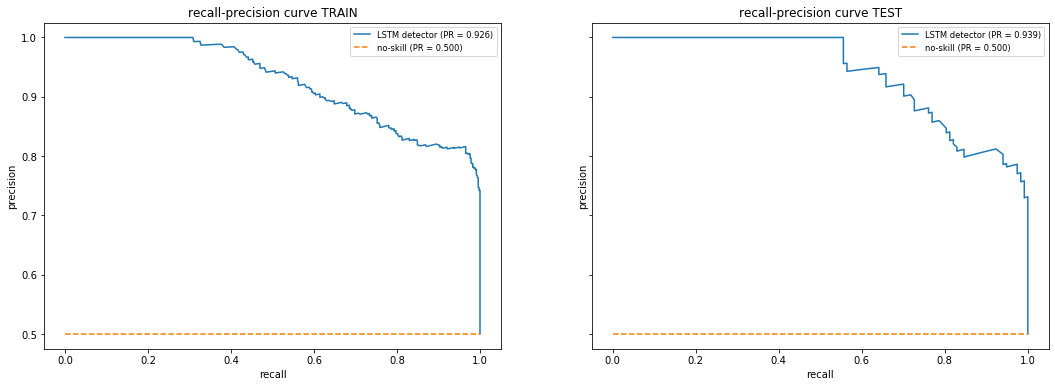
\includegraphics[width=1.\textwidth]{pr-train-test}
  \caption{Curvas sensibilidad-precisión en \emph{train} y \emph{test}.}
  \label{fig:ad-pr-train-test}
\end{figure}

Vemos por los resultados de la métrica y comparando con el clasificador base que nuestro detector se comporta bastante bien, obteniendo una puntuación bastante elevada. Observamos que podemos obtener una sensibilidad muy alta a costa de perder muy poca precisión, en cualquier caso el umbral usado dependería del problema real concreto.

\subsubsection{Alteraciones}

Procedemos a crear muestras anómalas con nuestros métodos, aunque como hemos visto en el patrón de la serie no parece que haya una componente cíclica clara, por lo que no usaremos los métodos de descomposición STL.

Empezaremos por el \textbf{ruido gaussiano}, donde aplicamos perturbaciones con tamaños entre $[3, 11]$ y $\sigma$ en $\{0.75, 0.9, 1, 1.25\}$. Tanto en tamaño como en $\sigma$ tenemos unos valores bastantes bajos para que las alteraciones sean muy leves y poner a prueba el modelo.

Mostramos 4 ejemplos para cada $\sigma$ en \autoref{fig:ad-gauss-1}, \autoref{fig:ad-gauss-2}, \autoref{fig:ad-gauss-3} y \autoref{fig:ad-gauss-3}.

\begin{figure}[htpb]
  \centering
  %\hspace*{-2.5cm}
  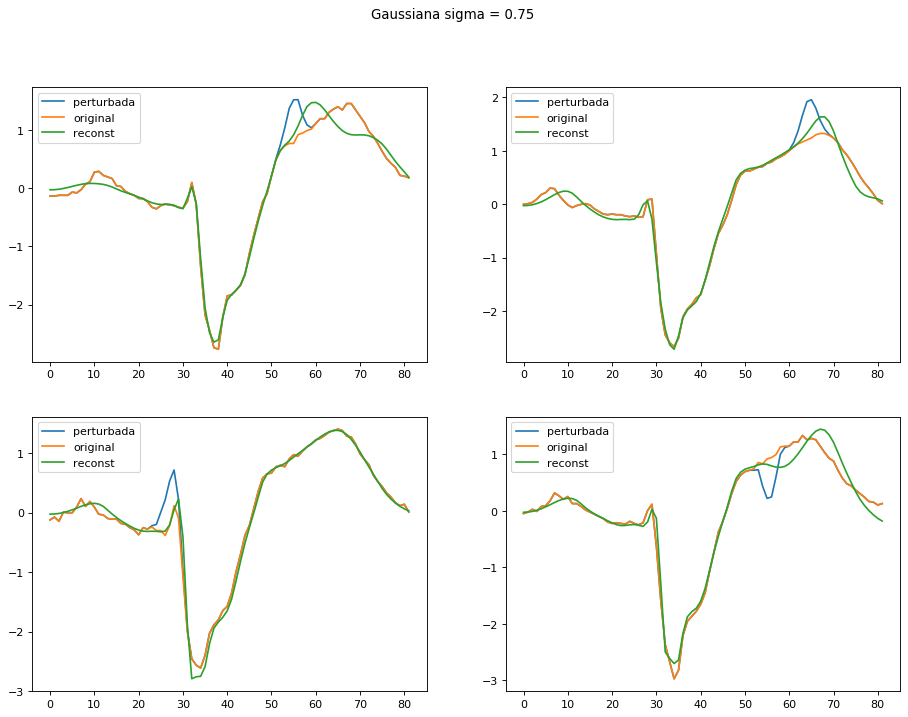
\includegraphics[width=.8\textwidth]{gauss-1}
  \caption{Alteraciones con ruido gaussiano a $\sigma = 0.75$.}
  \label{fig:ad-gauss-1}
\end{figure}

\begin{figure}[htpb]
  \centering
  %\hspace*{-2.5cm}
  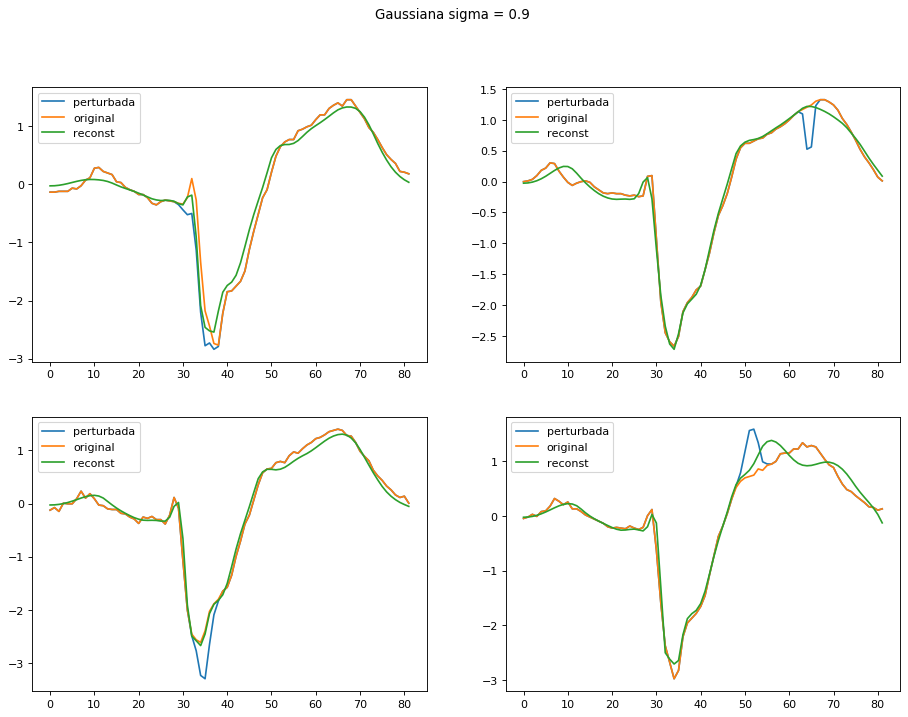
\includegraphics[width=.8\textwidth]{gauss-2}
  \caption{Alteraciones con ruido gaussiano a $\sigma = 0.9$.}
  \label{fig:ad-gauss-2}
\end{figure}

\begin{figure}[htpb]
  \centering
  %\hspace*{-2.5cm}
  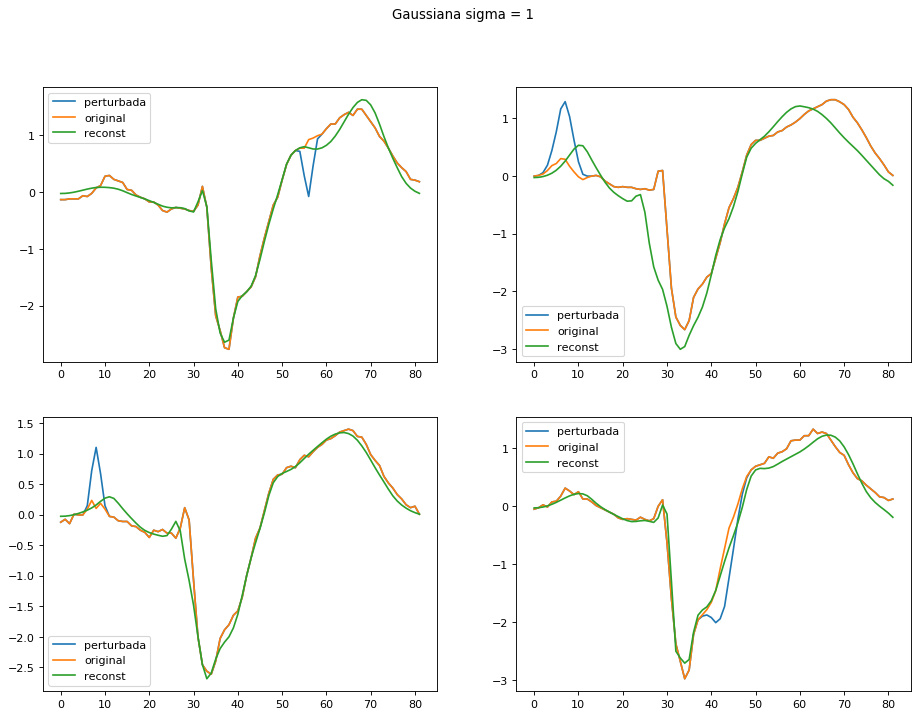
\includegraphics[width=.8\textwidth]{gauss-3}
  \caption{Alteraciones con ruido gaussiano a $\sigma = 1$.}
  \label{fig:ad-gauss-3}
\end{figure}

\begin{figure}[htpb]
  \centering
  %\hspace*{-2.5cm}
  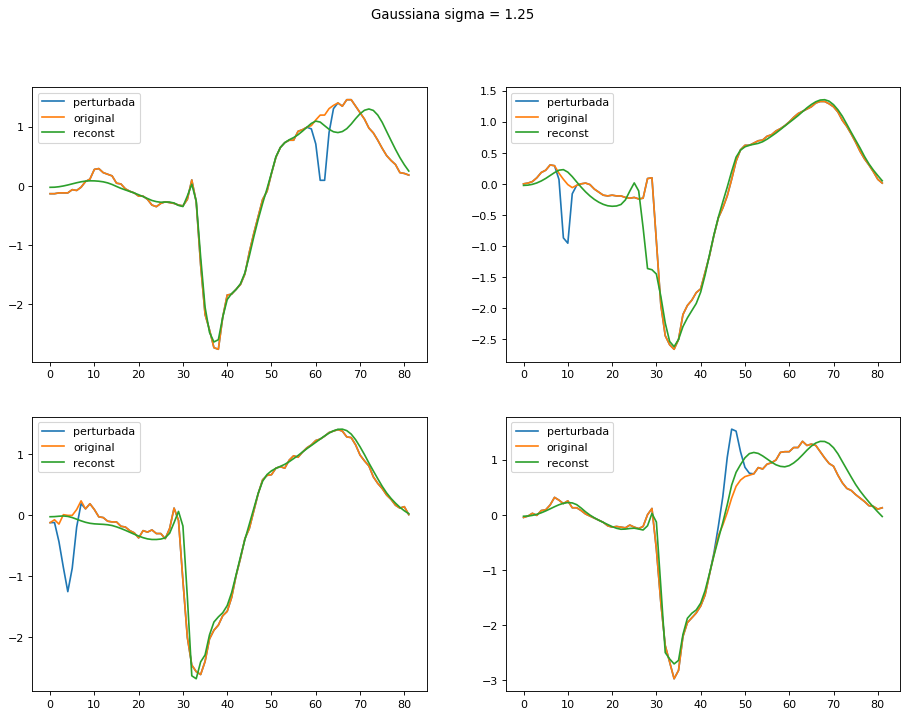
\includegraphics[width=.8\textwidth]{gauss-4}
  \caption{Alteraciones con ruido gaussiano a $\sigma = 1.25$.}
  \label{fig:ad-gauss-4}
\end{figure}

Observamos que generalmente las reconstrucciones son buenas hasta que llega al tramo de la perturbación, a partir de ahí la señal construida empieza a comportarse de manera muy distinta a la señal original añadiendo más error que permita identificar a la señal como anómala.

También notamos que la mayoría de perturbaciones no son especialmente bruscas, incluso según con la posición de la alteración, a veces no se diferencia casi nada
de la serie original.

Ahora pongamos a validar el modelo con la métrica $PR$, para ello crearemos tanto para \emph{train} como para \emph{test} una parte de anomalías con tamaño proporcional a cada uno, respectivamente. Tomaremos los ratios $\{0.05, 0.1, 0.2, 0.3\}$ para ver cuál es el efecto con muy pocas muestras y aumentando hasta que el tamaño de anomalías sea representativo de las posibles perturbaciones que se pueden aplicar. Finalmente por cada ratio tomaremos los $sigma$ en $\{0.75, 0.9, 1, 1.25\}$ para notar la diferencias a distinta escala.

Los resultados de \emph{train} los tenemos en \autoref{fig:ad-gauss-train} y de \emph{test} en \autoref{fig:ad-gauss-test}.

\begin{figure}[htpb]
  \centering
  %\hspace*{-2.5cm}
  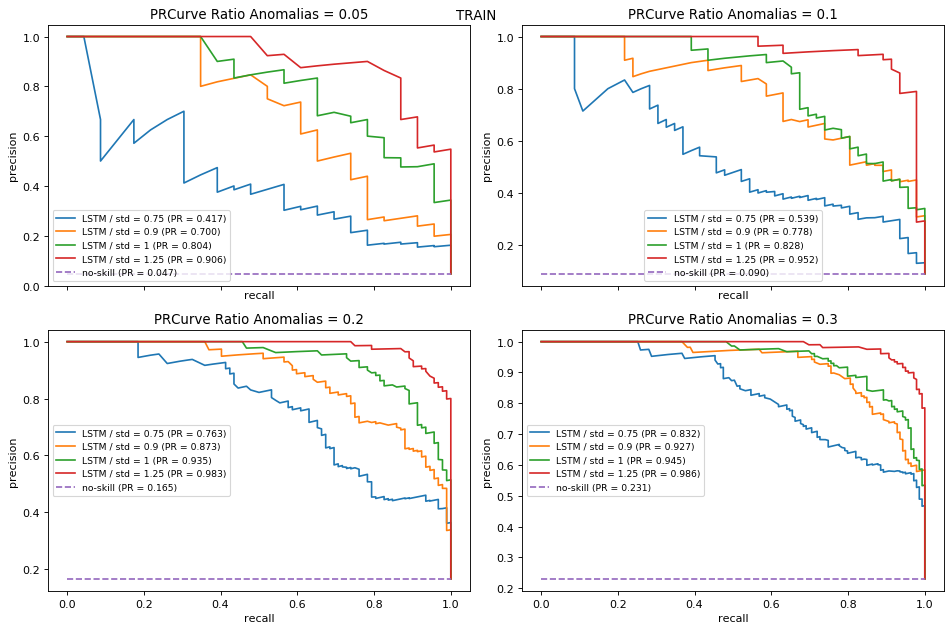
\includegraphics[width=.9\textwidth]{gauss-train}
  \caption{Curvas Sensibilidad-Precisión para distintas proporciones de número de anomalías y de intensidad con ruido gaussiano en \emph{train}.}
  \label{fig:ad-gauss-train}
\end{figure}

\begin{figure}[htpb]
  \centering
  %\hspace*{-2.5cm}
  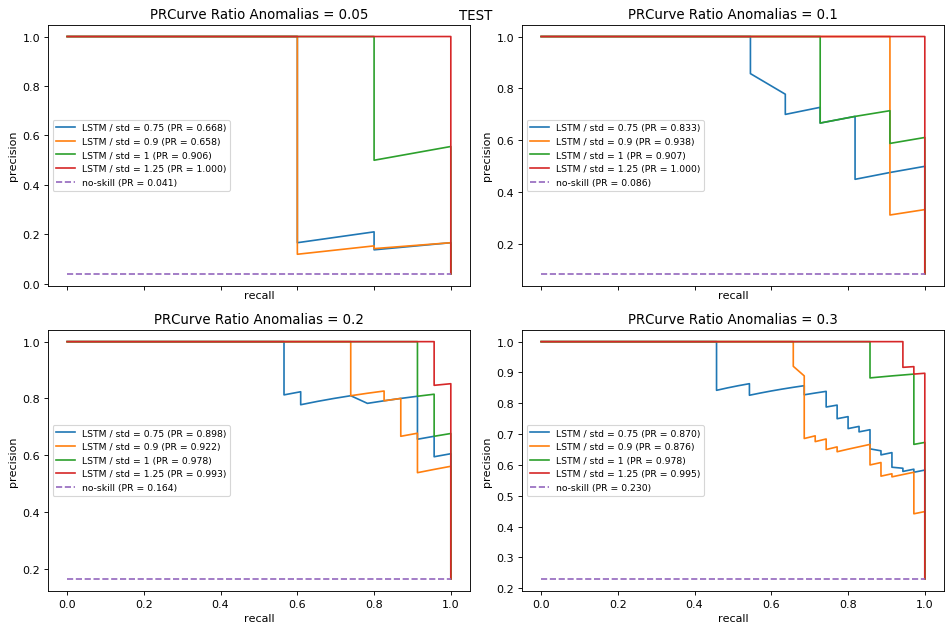
\includegraphics[width=.9\textwidth]{gauss-test}
  \caption{Curvas Sensibilidad-Precisión para distintas proporciones de número de anomalías y de intensidad con ruido gaussiano en \emph{test}.}
  \label{fig:ad-gauss-test}
\end{figure}

Se refleja claramente que a cuanta mayor proporción de anomalías mejor se comporta el modelo (mayor valores de $PR$), aunque probablemente se estabilice entre $[0.2, 0.3]$ que probablemente se deba a la aleatoriedad existente a la hora de escoger la posición y la longitud de la perturbación. También parece que conforme es más intensa la perturbación no parece influir tanto el ratio.

En cualquiera de los casos, todos los resultados indican que el modelo se comporta mejor que el clasificador base (tanto visualmente como con valores de la métrica) por lo que por lo menos el detector funciona en cierta manera. Los peores resultados que puede que se vean están en \emph{test} con $0.05$ pero seguramente debido a que son muy pocas anomalías.

Viendo el comportamiento más estable en los ratios de $0.2$ y $0.3$ queda constatado que el modelo es capaz de detectar bastante bien estas pequeñas anomalías en las escalas más pequeñas que hemos visto que son bastante suaves. Cuando la escala ya empieza a a ser más evidente, pero sin ser picos exageradamente grandes, el detector consigue valores de la métrica casi perfectos.

Vistos los resultados del ruido, pasamos al \textbf{pulso gaussiano-sinusoidal}, donde operamos de la misma manera que antes, aplicando perturbaciones con tamaño $[5, 11]$ (para que se vea la forma de la señal) y $\sigma$ en $\{0.75, 0.9, 1, 1.25\}$ que van desde pequeñas alteraciones a más obvias.

Mostramos 4 ejemplos para cada $\sigma$ en \autoref{fig:ad-pulso-1}, \autoref{fig:ad-pulso-2}, \autoref{fig:ad-pulso-3} y \autoref{fig:ad-pulso-3}.

\begin{figure}[htpb]
  \centering
  %\hspace*{-2.5cm}
  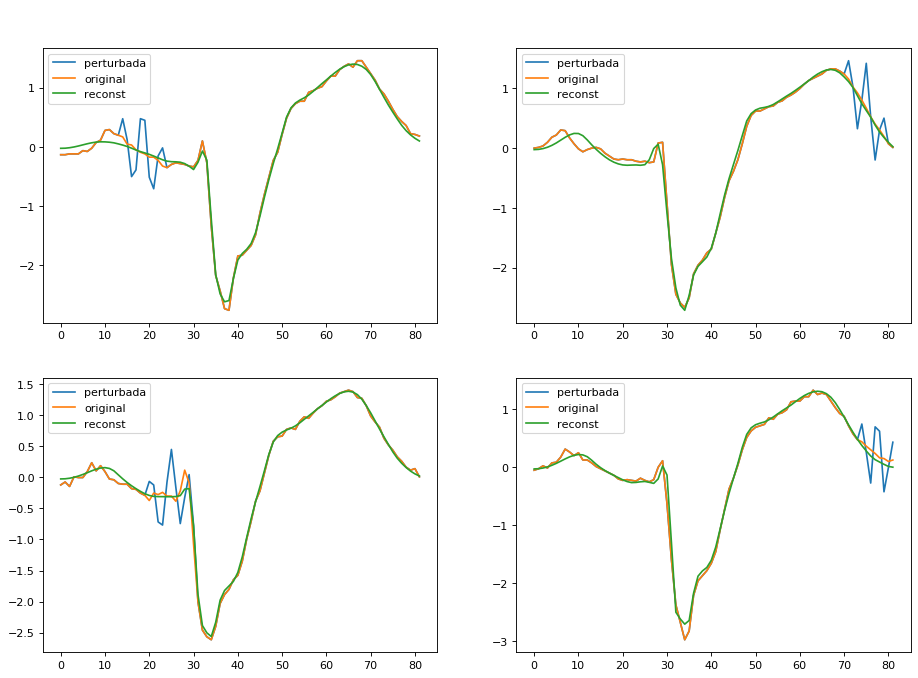
\includegraphics[width=.8\textwidth]{pulso-1}
  \caption{Alteraciones con pulso gaussiano-sinusoidal a $\sigma = 0.75$.}
  \label{fig:ad-pulso-1}
\end{figure}

\begin{figure}[htpb]
  \centering
  %\hspace*{-2.5cm}
  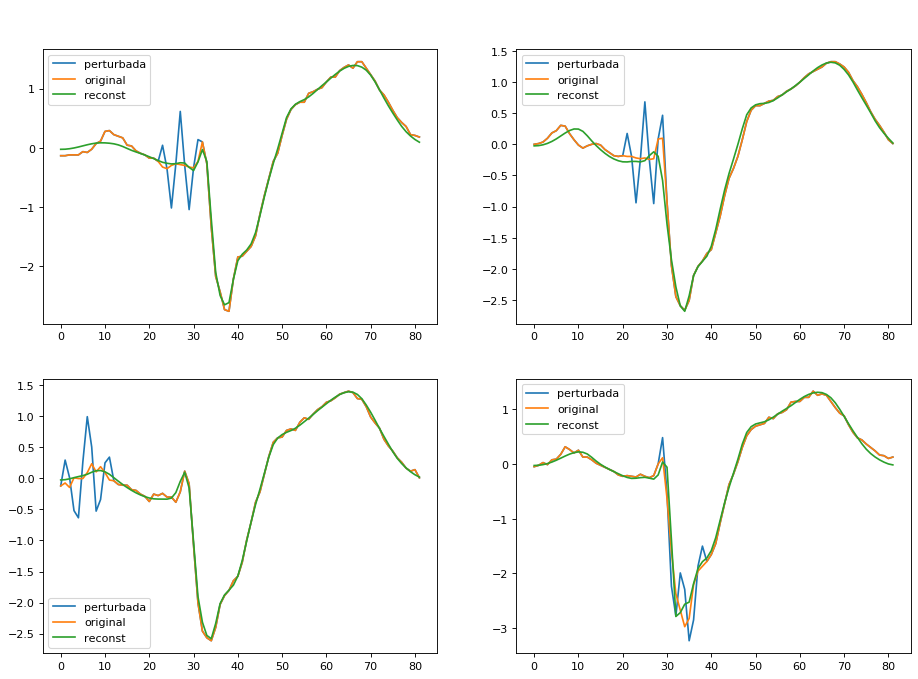
\includegraphics[width=.8\textwidth]{pulso-2}
  \caption{Alteraciones con pulso gaussiano-sinusoidal a $\sigma = 0.9$.}
  \label{fig:ad-pulso-2}
\end{figure}

\begin{figure}[htpb]
  \centering
  %\hspace*{-2.5cm}
  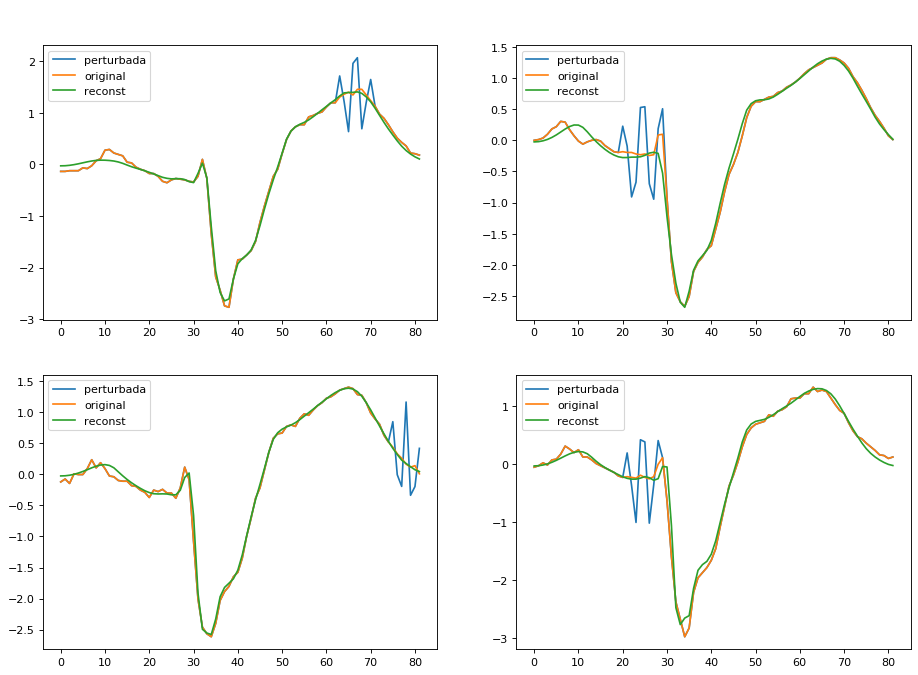
\includegraphics[width=.8\textwidth]{pulso-3}
  \caption{Alteraciones con pulso gaussiano-sinusoidal a $\sigma = 1$.}
  \label{fig:ad-pulso-3}
\end{figure}

\begin{figure}[htpb]
  \centering
  %\hspace*{-2.5cm}
  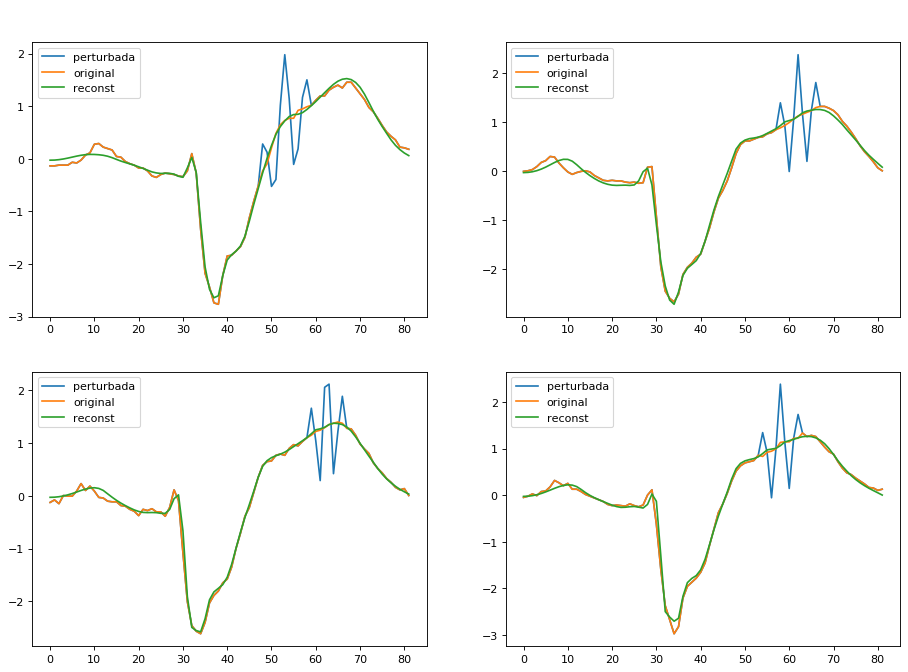
\includegraphics[width=.8\textwidth]{pulso-4}
  \caption{Alteraciones con pulso gaussiano-sinusoidal a $\sigma = 1.25$.}
  \label{fig:ad-pulso-4}
\end{figure}

Se aprecia correctamente los pulsos que cambian la forma de la señal, sin tener unos cambios muy bruscos en el rango de valores de la señal original, notándose más cuando $\sigma = 1.25$. También es digno de notar que, a diferencia con el ruido gaussiano, aquí las alteraciones cambian poco la reconstrucción debiéndose quizás al carácter sinusoidal de la perturbación aunque no podemos asegurar nada.

Repetimos de nuevo el cálculo del $PR$ con los mismos tamaños, escalas de $\sigma$ y ratios de proporción; obteniendo \autoref{fig:ad-pulso-train} en \textbf{train} y \autoref{fig:ad-pulso-test} en \emph{test}.

\begin{figure}[htpb]
  \centering
  %\hspace*{-2.5cm}
  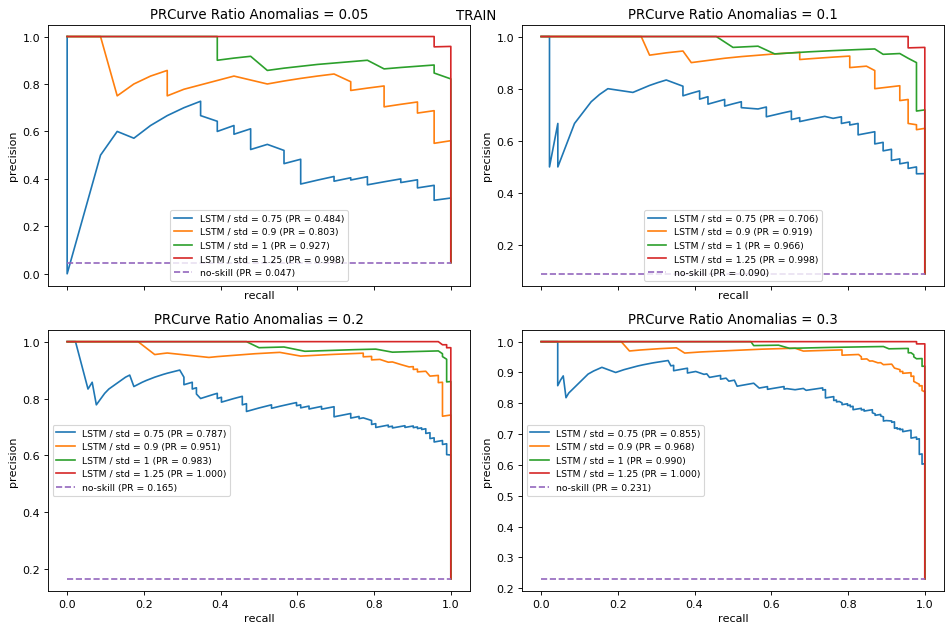
\includegraphics[width=.85\textwidth]{pulso-train}
  \caption{Curvas Sensibilidad-Precisión para distintas proporciones de número de anomalías y de intensidad con pulso gaussiano-sinusoidal en \emph{train}.}
  \label{fig:ad-pulso-train}
\end{figure}

\begin{figure}[htpb]
  \centering
  %\hspace*{-2.5cm}
  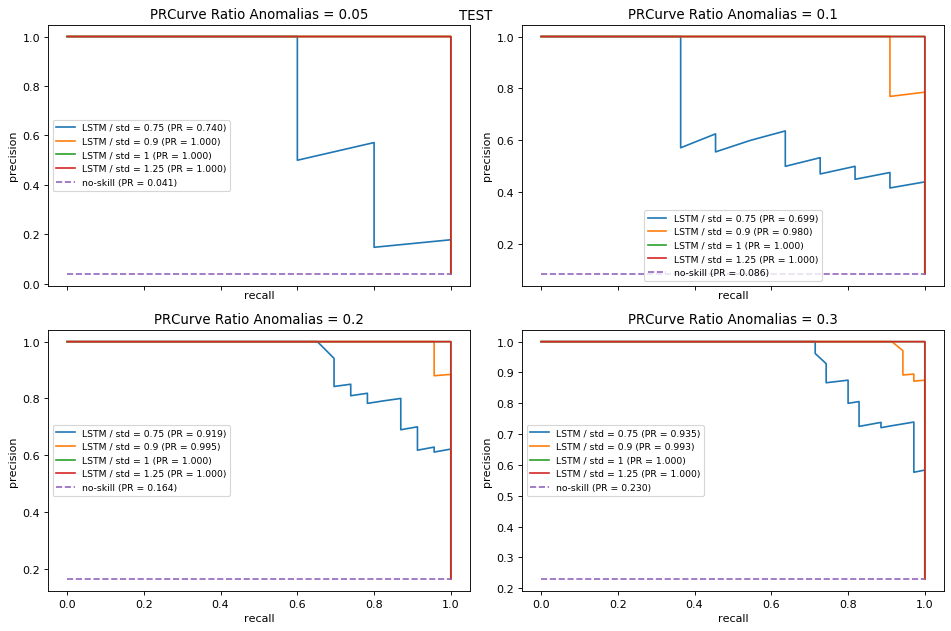
\includegraphics[width=.85\textwidth]{pulso-test}
  \caption{Curvas Sensibilidad-Precisión para distintas proporciones de número de anomalías y de intensidad con pulso gaussiano-sinusoidal en \emph{test}.}
  \label{fig:ad-pulso-test}
\end{figure}

El comportamiento respecto el ratio es igual que el ruido gaussiano, da mejores resultados con mejor ratio, aunque se nota que menos la escala más pequeña de $\sigma$ el resto obtienen muy buenos resultados casi perfectos notándose más exageradamente en \emph{test}.

Los resultados vuelven a indicar que el detector consigue realizar un buen trabajo a todas las escalas y con muy pocas muestras anómalas, de hecho parece que se consiguen muchos mejores resultados que el ruido gaussiano, aunque también puede deberse a que hayamos aumentado el tamaño mínimo de las perturbaciones.

Cuando la escala es la más pequeña ($\sigma = 0.75$) se comporta bastante peor aunque solo con con el menor ratio. Sin embargo, no es de extrañar puesto que aunque estemos fluctuando la forma de la señal en esa escala los cambios son muy pequeños y no se diferencian demasiado de la original. A pesar de todo esto el sistema es capaz de hacer un buen trabajo frente al clasificador base y va mejorando bastante las puntuaciones con mayor proporción de anomalías.

Resumiendo, el sistema es capaz de detectar bastante bien las clases existentes que habíamos clasificado como anómalas y también las alteraciones artificiales que hemos creado a distintas escalas, tamaños y proporciones; indicando el buen rendimiento de este detector.

\section{Dataset sintético}

\subsection{Descripción}

Para demostrar los métodos basados en descomposición STL, usaremos el \emph{dataset} basado en funciones coseno que habíamos creado a modo de ejemplo anteriormente. Recordamos que muestreábamos una función coseno, le añadíamos tendencia ascendente y ruido blanco; finalmente se estandarizaban. Volvemos a dejar un 20\% para \emph{test}.

Inspeccionamos 10 series del \emph{dataset}  para ver si hay un patrón, aunque ya sabemos que sí lo va a haber. En \autoref{fig:ad-dataset-cosenos} vemos claramente el patrón, aunque observamos el ruido introducido provoca pequeñas oscilaciones.

\begin{figure}[htpb]
  \centering
  %\hspace*{-2.5cm}
  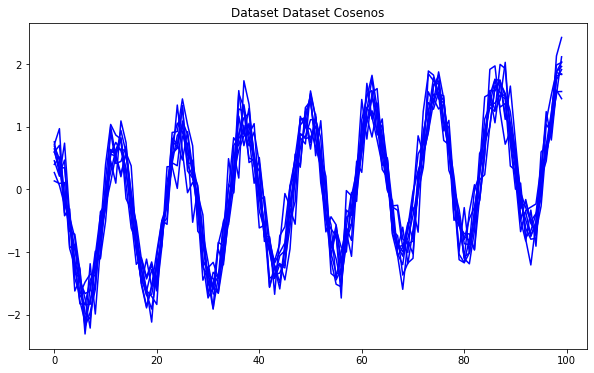
\includegraphics[width=.7\textwidth]{dataset-cos}
  \caption{Algunas series del \emph{dataset} \emph{Cosenos}.}
  \label{fig:ad-dataset-cosenos}
\end{figure}

\subsection{Entrenamiento}

Repetimos usando el modelo que teníamos entrenando durante 400 épocas con un número de neuronas a $[20, 10, 10, 20]$ (la función es muy sencilla por lo que necesitamos muchas neuronas), sin regularización, con tasa de aprendizaje de $0.001$, tamaño de \emph{batch} de 128 y con un conjunto de validación usando el 10\%.

El resultado del entrenamiento mostrando la función de pérdida MSE se muestra en \autoref{fig:ad-entrenamiento-cos}. Nos muestra que no hay sobreajuste puesto que ambas curvas van unidas y el entrenamiento es correcto puesto que el error baja casi a 0; en este caso hemos entrenado muchas épocas para bajar al máximo posible los errores.

\begin{figure}[htpb]
  \centering
  %\hspace*{-2.5cm}
  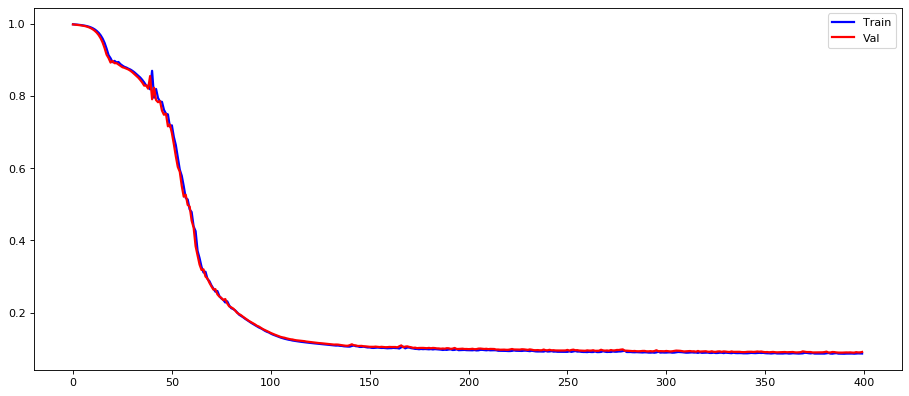
\includegraphics[width=.8\textwidth]{train-cos}
  \caption{Entrenamiento del modelo LSTM en \emph{Cosenos}.}
  \label{fig:ad-entrenamiento-cos}
\end{figure}

Observemos algunas series en \emph{train} y \emph{test} con varias reconstrucciones para ver el comportamiento del modelo en \autoref{fig:ad-reconstruccion-cos-train} y \autoref{fig:ad-reconstruccion-cos-test} respectivamente.

\begin{figure}[htpb]
  \centering
  %\hspace*{-2.5cm}
  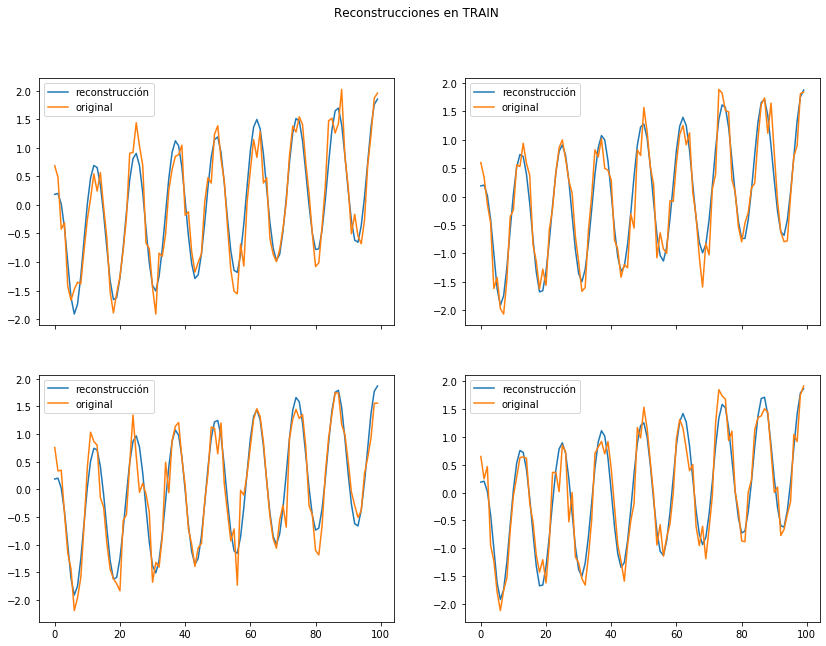
\includegraphics[width=.8\textwidth]{cos-reconst-train}
  \caption{Reconstrucciones en \emph{train}.}
  \label{fig:ad-reconstruccion-cos-train}
\end{figure}

\begin{figure}[htpb]
  \centering
  %\hspace*{-2.5cm}
  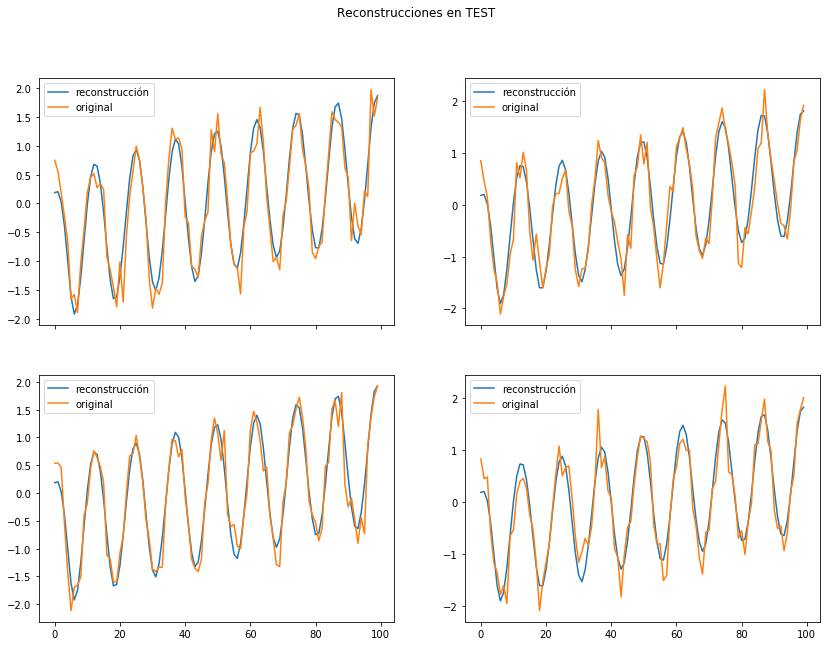
\includegraphics[width=.8\textwidth]{cos-reconst-test}
  \caption{Reconstrucciones en \emph{test}.}
  \label{fig:ad-reconstruccion-cos-test}
\end{figure}

Las reconstrucciones parecen bastante buenas ya que aprenden el modelo sinusoidal subyacente sin el ruido blanco, las diferencias que observamos son generalmente debidas a esto por lo que podemos considerar que el modelo ha aprendido correctamente el patrón de los datos.

Estudiamos ahora la distribución de errores MSE entre las series y las reconstrucciones en \emph{train} y \emph{test} en \autoref{fig:ad-hist-cos}, junto con la estimación de la función de densidad.

\begin{figure}[htpb]
  \centering
  %\hspace*{-2.5cm}
  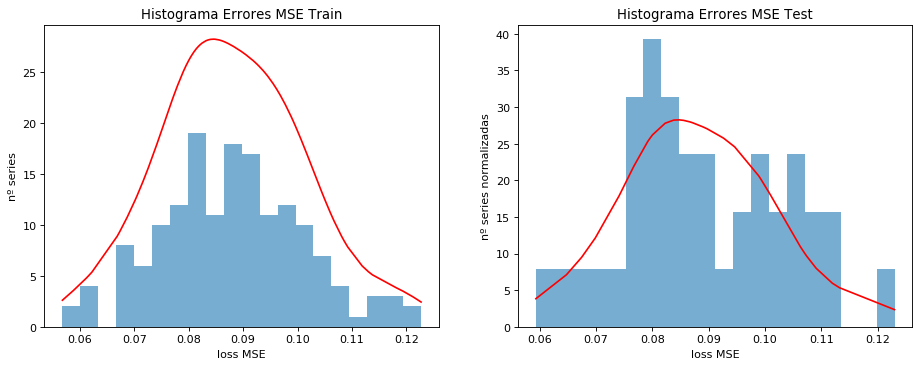
\includegraphics[width=1.\textwidth]{cos-hists}
  \caption{Histogramas de error en \emph{train} y \emph{test}.}
  \label{fig:ad-hist-cos}
\end{figure}

Como habíamos visto que el modelo había aprendido correctamente el patrón, los errores esperados se comportan como una gaussiana, es decir como ruido blanco por lo que probablemente no queda más que pueda extraer el modelo. El comportamiento en \emph{train} y \emph{test} es el mismo, por lo que hace una buena generalización.

Habiendo obtenido la función de densidad estimada, el modelo ya ha sido entrenado y listo para poner a prueba frente a las alteraciones.

\subsection{Validación}

Para este conjunto de datos usaremos la validación usando las alteraciones basadas en la descomposición STL para comprobar su eficacia y a la vez el rendimiento del detector ante este tipo de anomalías.

Volvemos a usar como métrica $PR$ para valorar el modelo.

\subsubsection{Estacionalidad}

Empezamos a crear anomalías alterando la componente de la \textbf{estacionalidad} de las series con tamaños entre $[7, 11]$ y $\sigma$ en $\{0.01, 0.05, 1.8, 2.0\}$ para que se aprecien las alteraciones en al menos medio periodo y para amortiguar la estacionalidad ($\sigma < 1$) y amplificarla ($\sigma > 1$).

Mostramos 4 ejemplos para cada $\sigma$ en \autoref{fig:ad-season1}, \autoref{fig:ad-season2}, \autoref{fig:ad-season3} y \autoref{fig:ad-season4} respectivamente.

\begin{figure}[htpb]
  \centering
  %\hspace*{-2.5cm}
  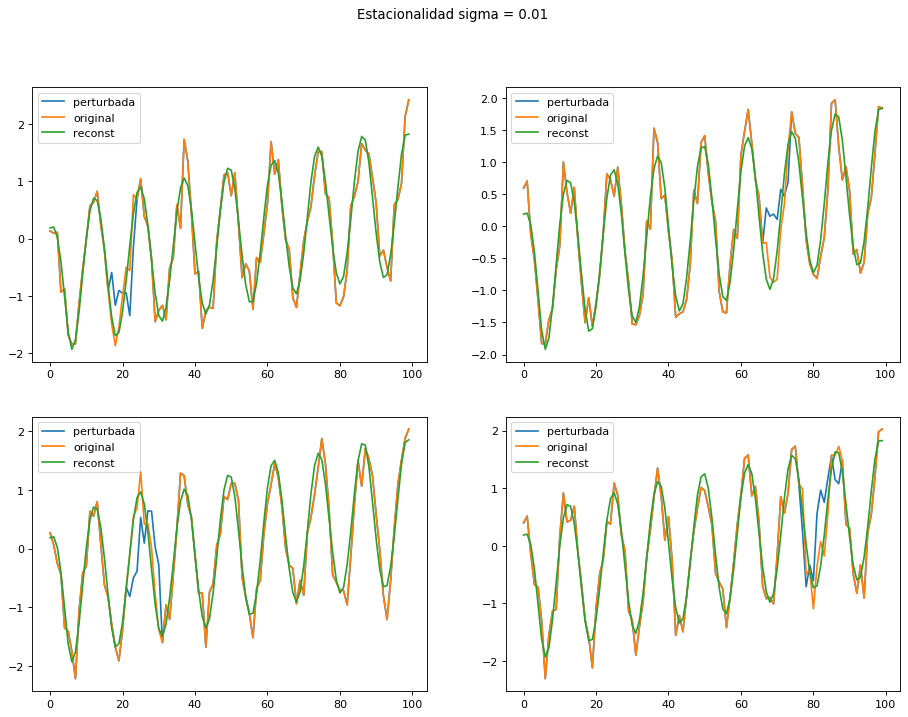
\includegraphics[width=.8\textwidth]{season1}
  \caption{Modificación de la estacionalidad a $\sigma = 0.01$.}
  \label{fig:ad-season1}
\end{figure}

\begin{figure}[htpb]
  \centering
  %\hspace*{-2.5cm}
  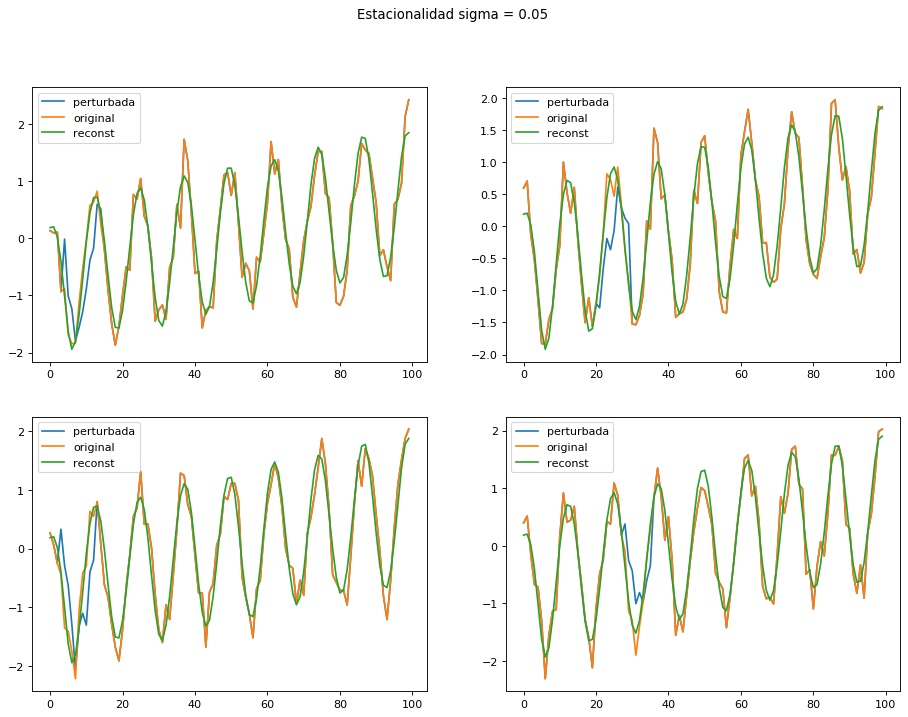
\includegraphics[width=.8\textwidth]{season2}
  \caption{Modificación de la estacionalidad a $\sigma = 0.05$.}
  \label{fig:ad-season2}
\end{figure}

\begin{figure}[htpb]
  \centering
  %\hspace*{-2.5cm}
  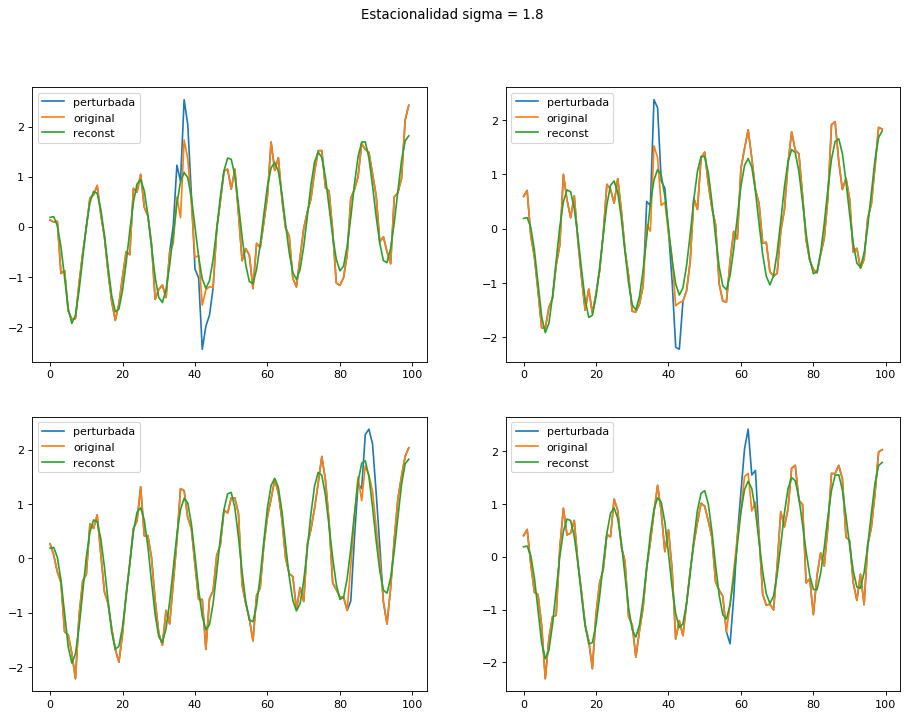
\includegraphics[width=.8\textwidth]{season3}
  \caption{Modificación de la estacionalidad a $\sigma = 1.8$.}
  \label{fig:ad-season3}
\end{figure}

\begin{figure}[htpb]
  \centering
  %\hspace*{-2.5cm}
  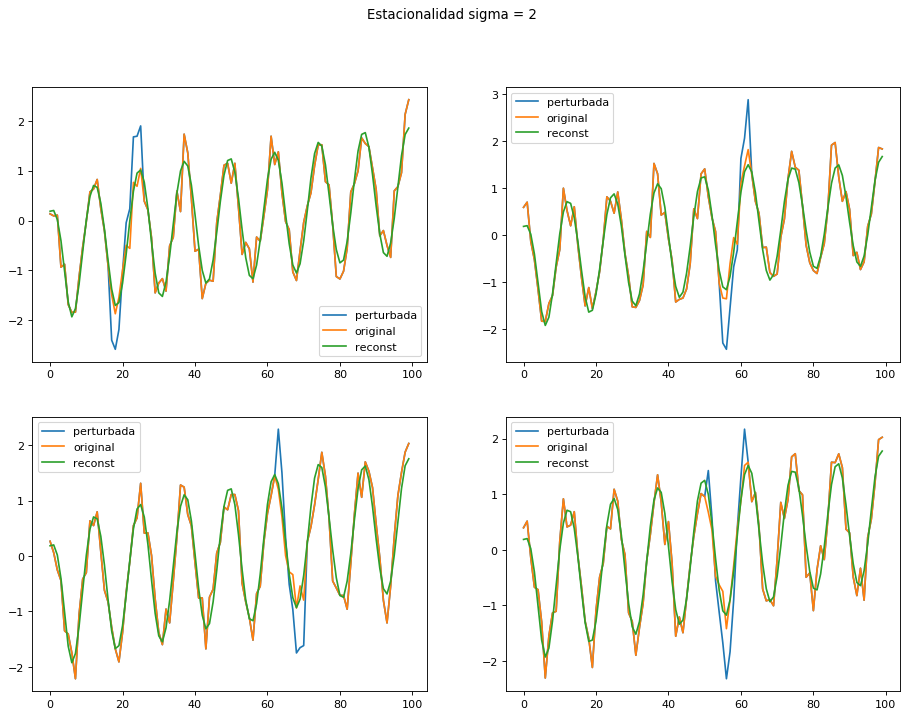
\includegraphics[width=.8\textwidth]{season4}
  \caption{Modificación de la estacionalidad a $\sigma = 2$.}
  \label{fig:ad-season4}
\end{figure}

Conseguimos el efecto deseado: para $\sigma < 1$ amortiguamos la estacionalidad y para $\sigma > 1$ se amplifica, modificando la serie de una manera sinusoidal debido al carácter propio de su estacionalidad. La reconstrucción se mantiene casi sin alteraciones por lo que queda en evidencia clara la anomalía que se muestra, aunque debido al ruido que había en el \emph{dataset} no es fácil determinar si es una anomalía completamente.

Validemos calculando la métrica $PR$ de la misma manera que hicimos con el otro \emph{dataset}: tomando \emph{train} y \emph{test} y creando alteraciones con un número proporcional al tamaño de cada uno respectivamente, en concreto los ratios $\{0.05, 0.1, 0.2, 0.3\}$. La configuración de las alteraciones es la misma que la de los ejemplos.

Obtenemos los resultados de \emph{train} en \autoref{fig:ad-season-train} y \emph{test} en \autoref{fig:ad-season-test}.

\begin{figure}[htpb]
  \centering
  %\hspace*{-2.5cm}
  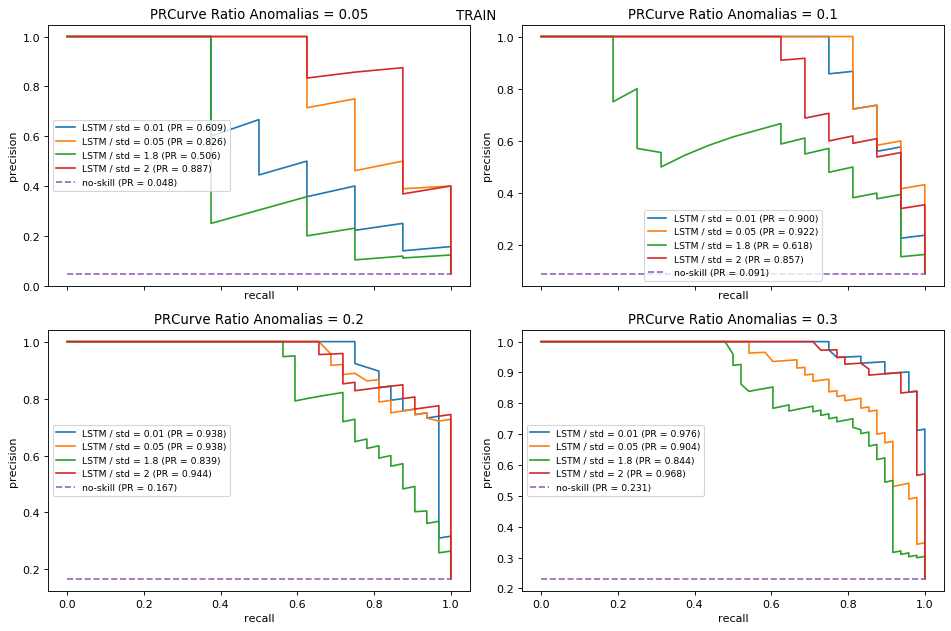
\includegraphics[width=.85\textwidth]{season-train}
  \caption{Curvas Sensibilidad-Precisión para distintas proporciones de número de anomalías y de intensidad modificando la estacionalidad en \emph{train}.}
  \label{fig:ad-season-train}
\end{figure}

\begin{figure}[htpb]
  \centering
  %\hspace*{-2.5cm}
  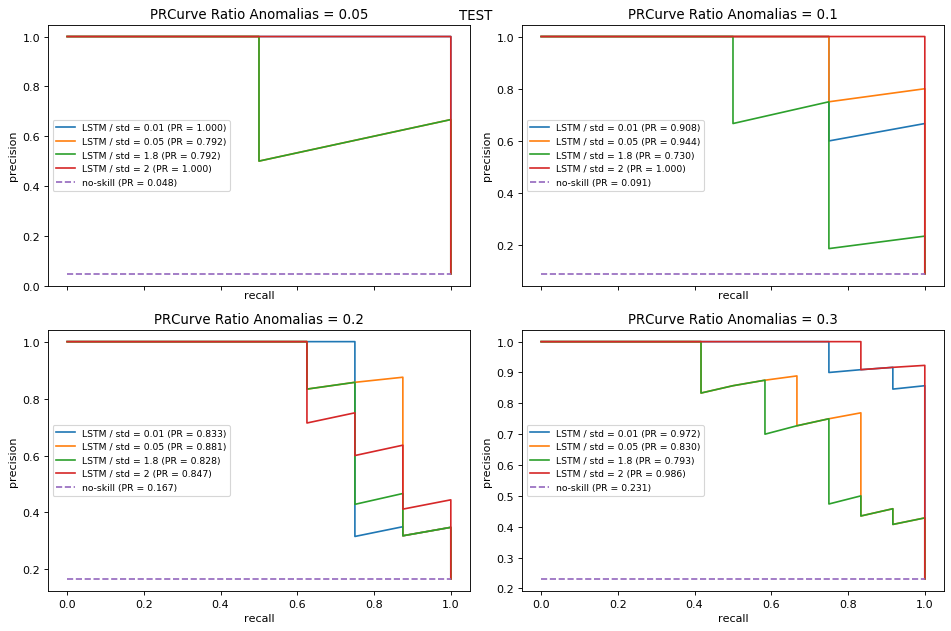
\includegraphics[width=.85\textwidth]{season-test}
  \caption{Curvas Sensibilidad-Precisión para distintas proporciones de número de anomalías y de intensidad modificando la estacionalidad en \emph{test}.}
  \label{fig:ad-season-test}
\end{figure}

Se obtiene un resultado parecido en el otro \emph{dataset}: conforme aumenta el número de perturbaciones los valores de las métricas van aumentando hasta estabilizarse; y en \emph{test} es un poco inestable con un ratio bajo debido al menor número de series.

En todos los casos el detector es capaz de obtener un rendimiento superior al clasificador aleatorio, consiguiendo tasas de la métrica muy elevadas desde un ratio del 0.1 por lo que podemos decir el modelo consigue detectar la mayoría de estas anomalías siendo realmente efectivo.

Para los $\sigma$ de amortiguación de señal vemos que el comportamiento es muy parecido entre los dos valores, en los de amplificación el valor $2$ parece que crea anomalías más obvias que $1.8$. En cualquier caso, las perturbaciones realizadas parecen ser casi como el ruido gaussiano que hemos introducido, siendo solo un poco más fuertes, y aun así el detector es capaz de detectarlas lo que nos indica la gran sensibilidad que tiene.

\subsubsection{Tendencia}

Repetimos lo que hemos hecho pero ahora modificando la componente de la \textbf{tendencia} de las series con tamaños entre $[7, 11]$ y $\sigma$ en $\{-1, 0.001, 3.5, 4\}$ que han sido tomados para invertir la tendencia ($\sigma < 0$), amortiguarla ($0 < \sigma < 1$) o amplificarla ($\sigma > 1$).

Mostramos 4 ejemplos para cada $\sigma$ en \autoref{fig:ad-trend1}, \autoref{fig:ad-trend2}, \autoref{fig:ad-trend3} y \autoref{fig:ad-trend4} respectivamente.

\begin{figure}[htpb]
  \centering
  %\hspace*{-2.5cm}
  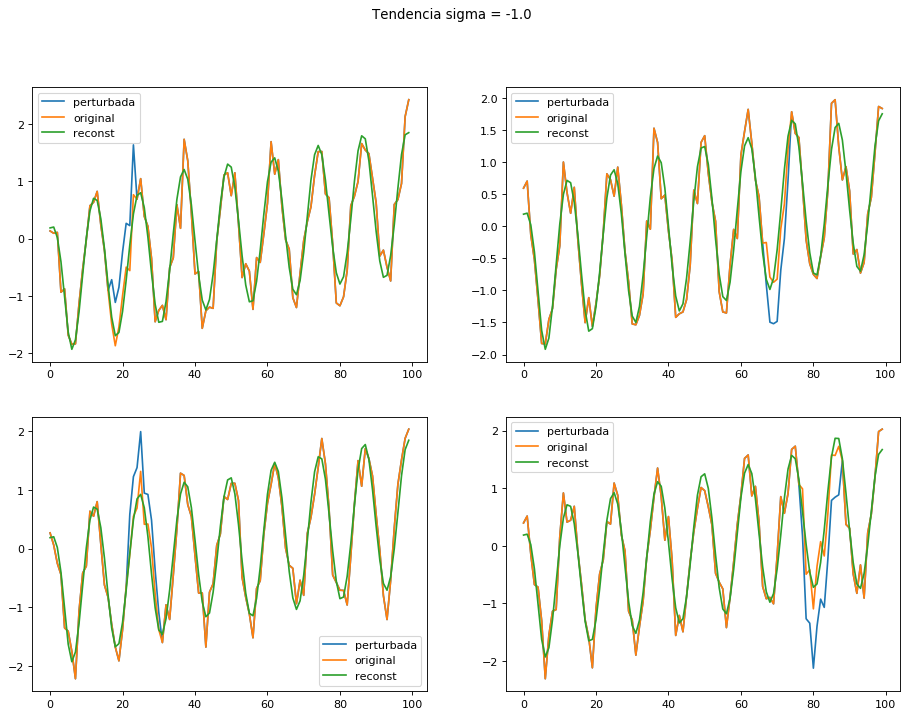
\includegraphics[width=.8\textwidth]{trend1}
  \caption{Modificación de la tendencia a $\sigma = -1$.}
  \label{fig:ad-trend1}
\end{figure}

\begin{figure}[htpb]
  \centering
  %\hspace*{-2.5cm}
  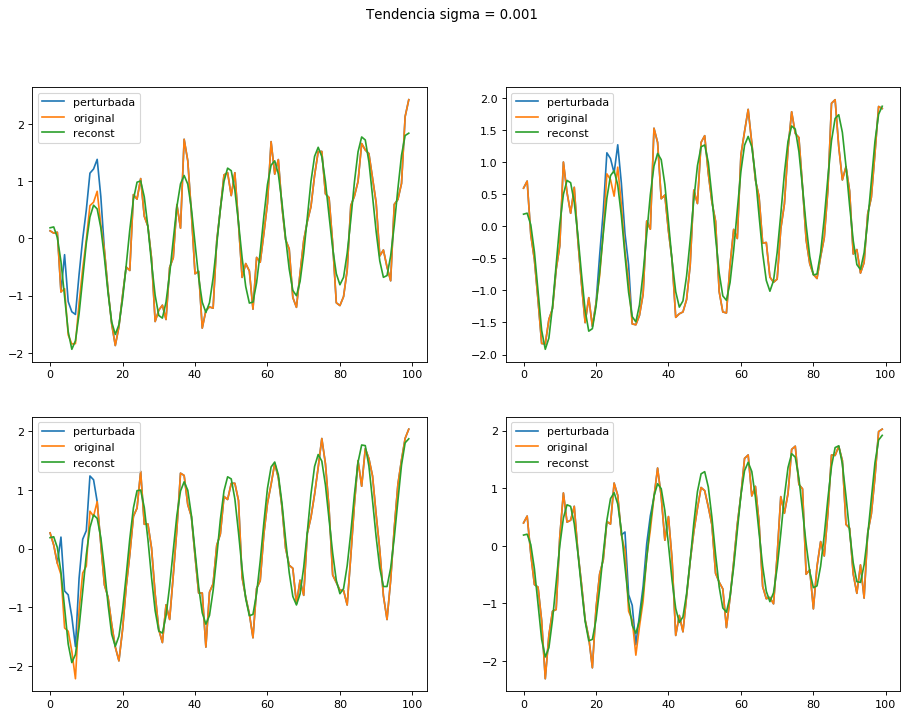
\includegraphics[width=.8\textwidth]{trend2}
  \caption{Modificación de la tendencia a $\sigma = 0.001$.}
  \label{fig:ad-trend2}
\end{figure}


\begin{figure}[htpb]
  \centering
  %\hspace*{-2.5cm}
  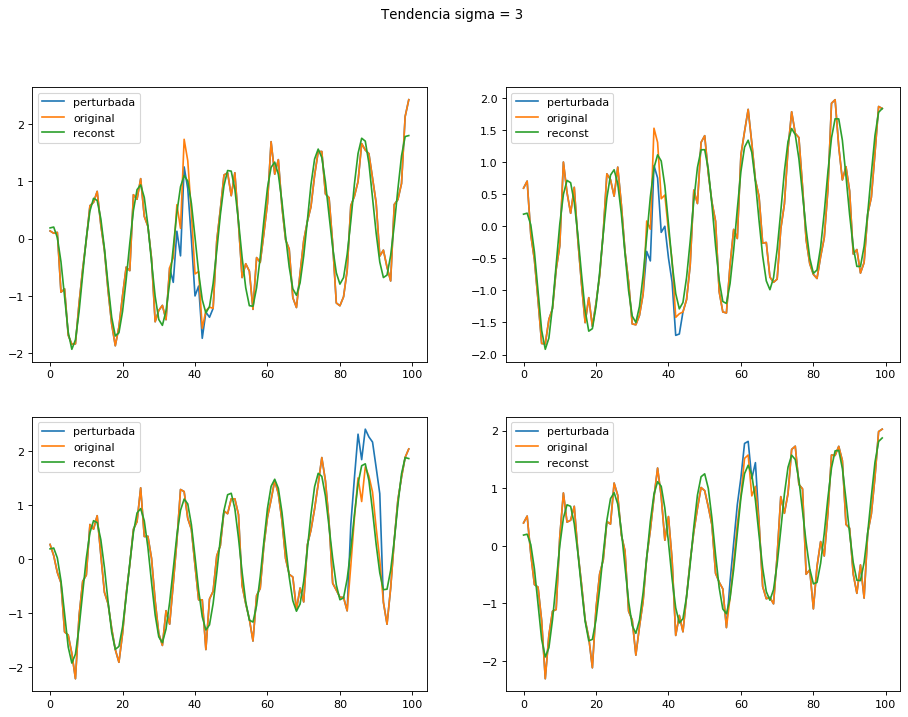
\includegraphics[width=.8\textwidth]{trend3}
  \caption{Modificación de la tendencia a $\sigma = 3$.}
  \label{fig:ad-trend3}
\end{figure}


\begin{figure}[htpb]
  \centering
  %\hspace*{-2.5cm}
  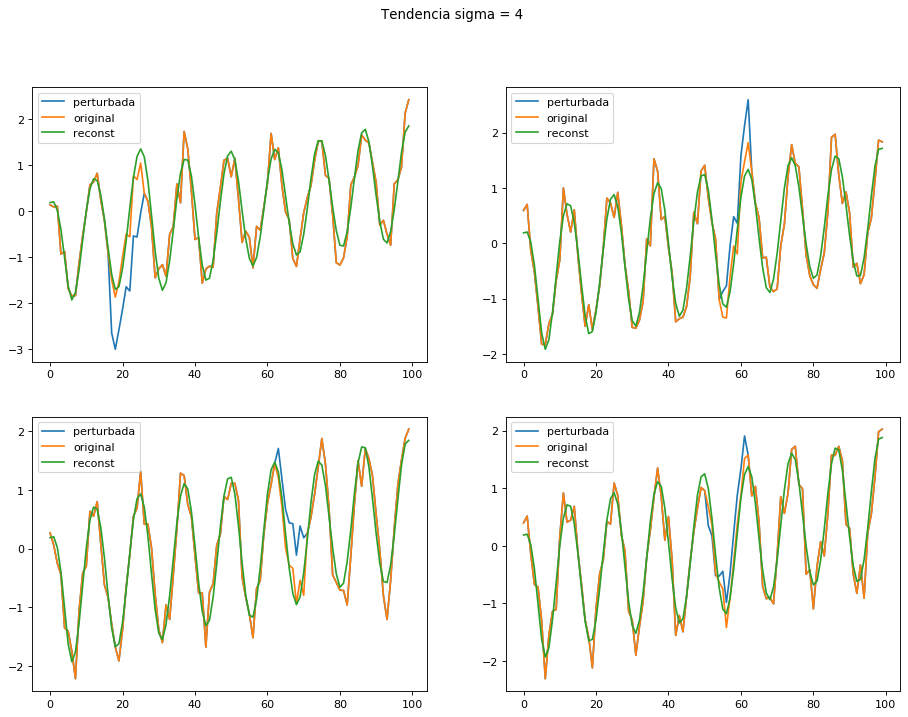
\includegraphics[width=.8\textwidth]{trend4}
  \caption{Modificación de la tendencia a $\sigma = 4$.}
  \label{fig:ad-trend4}
\end{figure}

Como en este caso la tendencia es como una recta que toma valores en $[-0.5, 0.5]$ las alteraciones se notarán más en los extremos ya que conforme nos acercamos al centro de las series la tendencia se anula, haciendo que cualquier variación sea imperceptible.

Con $\sigma = -1$ conseguimos invertir la tendencia y como vemos, en las zonas extremas de las series se puede notar más estas alteraciones; en todo caso como la tendencia no era muy grande en valor absoluto las modificaciones suelen ser pequeñitas.

Para $\sigma = 0.001$ amortiguamos la tendencia ocasionando que aumente en las zonas donde era negativa y disminuya para las positivas pero volvemos a notar que estas modificaciones son casi indistinguibles, parece que solo se aprecian en los extremos.

Con $\sigma = 3, 4$ amplificamos la tendencia pero volvemos a notar que las perturbaciones no se aprecian mucho aunque estas perturbaciones parecen ser más fuertes que el resto de casos.

Ahora pasamos a validar calculando la métrica $PR$ con la configuración anterior y los mismos ratios que hemos realizado anteriormente. Los resultados obtenidos de \emph{train} y \emph{test} están en \autoref{fig:ad-trend-train} y \autoref{fig:ad-trend-test} respectivamente.

\begin{figure}[htpb]
  \centering
  %\hspace*{-2.5cm}
  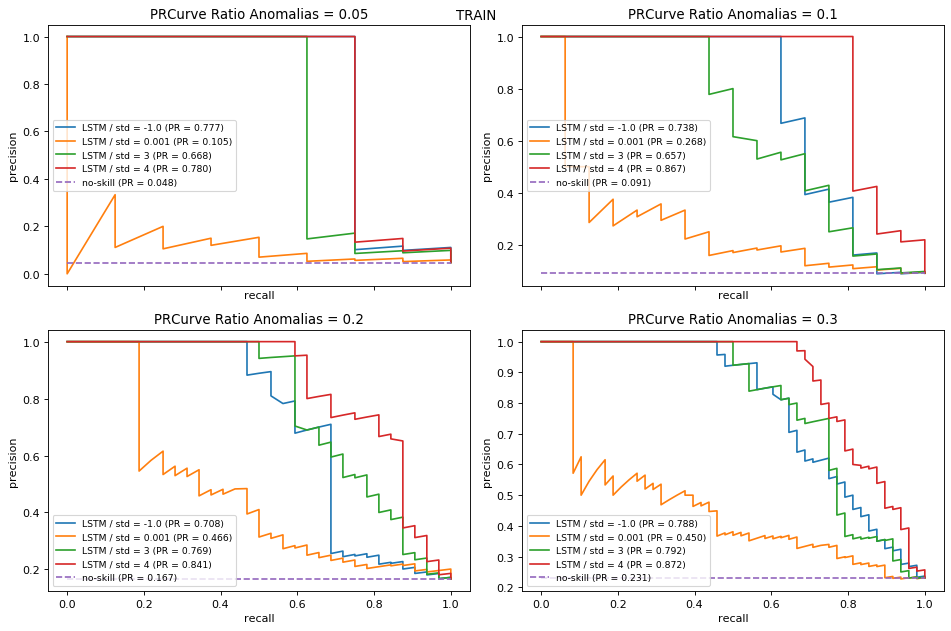
\includegraphics[width=.85\textwidth]{trend-train}
  \caption{Curvas Sensibilidad-Precisión para distintas proporciones de número de anomalías y de intensidad modificando la tendencia en \emph{train}.}
  \label{fig:ad-trend-train}
\end{figure}

\begin{figure}[htpb]
  \centering
  %\hspace*{-2.5cm}
  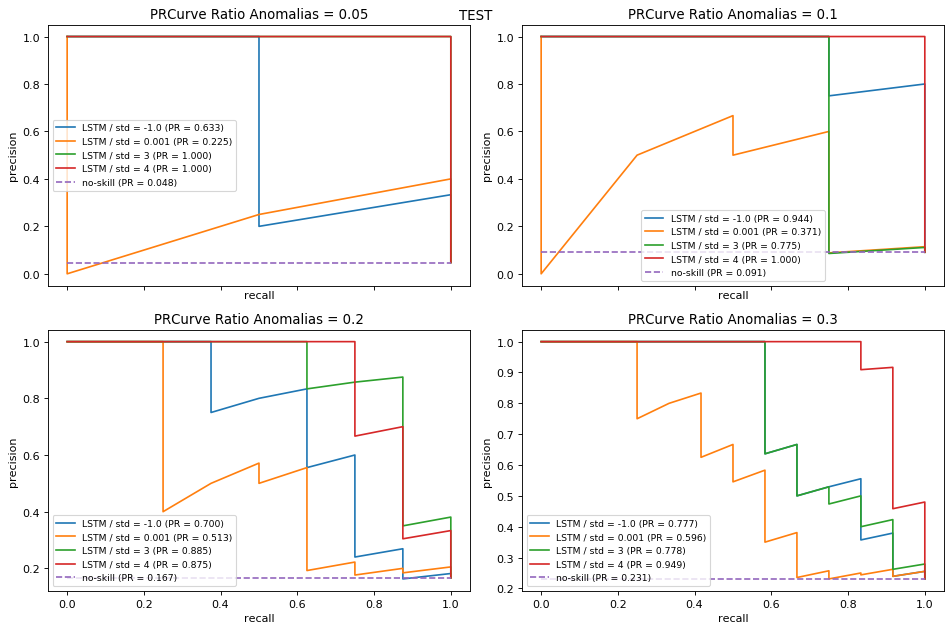
\includegraphics[width=.85\textwidth]{trend-test}
  \caption{Curvas Sensibilidad-Precisión para distintas proporciones de número de anomalías y de intensidad modificando la tendencia en \emph{test}.}
  \label{fig:ad-trend-test}
\end{figure}

Como era de esperar debido a que la tendencia se anula por el centro de las series, la mayoría de estas perturbaciones son casi imperceptibles y se nota debido a las caídas abruptas de las curvas, provocando así un comportamiento en general peor que el resto de alteraciones. Aun así, excepto $0.001$, para el resto de $\sigma$ el modelo es capaz de captar notablemente las alteraciones cuando el ratio de proporciones se estabiliza.

Destaca el peor rendimiento de $\sigma = 0.001$ aunque no es ninguna sorpresa, ya que las modificaciones muchas veces son casi imperceptibles debido a que puede mezclarse con ruido perfectamente o casi no hay efecto al estar cerca del centro. A pesar de ser el peor caso, el detector sigue realizando un mejor trabajo que el detector aleatorio.

\section{Resumen de resultados}

Resumimos todos los resultados del detector de anomalías y de los métodos de alteración aplicados: en general vemos que el detector se comporta muy bien a pesar de aplicar alteraciones que en ocasiones son indistinguibles del propio ruido blanco que pudiera aparecer en las series, obteniendo unos resultados excelentes cuando estas alteraciones empiezan a ser significativas.

Además se puede constatar la eficacia de los métodos para crear series anómalas, que variando la intensidad y la longitud según se desee para las series temporales concretas con las que se esté utilizando, se puede obtener resultados muy buenos para poder ser usados para múltiples propósitos como la propia validación de detectores.

También es cierto que las alteraciones que usan la descomposición STL son significativas cuando existe al menos una componente no nula de estacionalidad en las series, por lo que puede ser un poco restrictivo, y también puede que no sea muy efectivo cuando una de las componentes es relativamente pequeña respecto al resto (como pasa con la tendencia).

En cualquier caso, hemos comprobado visualmente con diversos ejemplos de estas series alteradas el funcionamiento correcto de estos métodos y el buen rendimiento del detector LSTM a la hora de detectar distintos tipos, con múltiples intensidades y tamaños, contrastado con el uso de la validación por partición en entrenamiento/test.




\endinput
%------------------------------------------------------------------------------------
% FIN DEL CAPÍTULO.
%------------------------------------------------------------------------------------
